%%%%%%%%%%%%%%%%%%%%%%%%%%%%% Thesis.tex %%%%%%%%%%%%%%%%%%%%%%%%%%%%%%%
%                                                                      %
%  ---------- Master of Science Dissertation template ----------       %
%                                                                      %
%  Template for the Master Thesis according to the regulations         %
%  published by the Academic Board (Direcção Académica) at IST.        %
%                                                                      %
%  For up-to-date guide, please refer to the official website          %
%  http://academica.tecnico.ulisboa.pt/alunos/dissertacao-de-mestrado/ %
%                                                                      %
%       Andre C. Marta                                                 %
%       Area Cientifica de Mecanica Aplicada e Aeroespacial            %
%       Departamento de Engenharia Mecanica                            %
%       Instituto Superior Tecnico                                     %
%       Av. Rovisco Pais                                               %
%       1049-001 Lisboa                                                %
%       Portugal                                                       %
%       Tel: +351 21 841 9469                                          %
%                        3469 (extension)                              %
%       Email: andre.marta@tecnico.ulisboa.pt                          %
%                                                                      %
%  Created:       Jan 20, 2011                                         %
%  Last Modified: Feb 19, 2018                                         %
%                                                                      %
%%%%%%%%%%%%%%%%%%%%%%%%%%%%%%%%%%%%%%%%%%%%%%%%%%%%%%%%%%%%%%%%%%%%%%%%
%  Revision history                                                    %
%  v1 - 2011/01/24 - original template                                 %
%  v2 - 2012/10/30 - new IST image and glossary support                %
%  v3 - 2013/12/10 - update according to 2012/13 official guide        %
%  v4 - 2014/02/28 - new default for bibliography style                %
%  v5 - 2014/05/07 - update according to 2013/14 official guide        %
%  v6 - 2015/07/02 - cover page format fixed,                          %
%                    contents page numbering fixed,                    %
%                    better language support,                          %
%                    enhanced examples of tables,                      %
%                    new option for appendix page numbering format,    %
%                    custom bibliography style                         %
%  v7 - 2018/02/19 - multiple citations compressed                     %
%%%%%%%%%%%%%%%%%%%%%%%%%%%%%%%%%%%%%%%%%%%%%%%%%%%%%%%%%%%%%%%%%%%%%%%%
%                                                                      %
% To generate the PDF file, type "make" at the terminal prompt.        %
%                                                                      %
% The IST template LaTeX package was created by the author             %
% and it can be downloaded from:                                       %
% https://fenix.ist.utl.pt/homepage/ist31052/                          %
%                                                                      %
% The external packages can be downloaded from                         %
% the Comprehensive TeX Archive Network at http://www.ctan.org/        %
%                                                                      %
% List of LaTex symbols:                                               %
% http://www.ctan.org/tex-archive/info/symbols/comprehensive/          %
%                                                                      %
% Help with LaTex can be found at                                      %
% http://www.giss.nasa.gov/tools/latex/ltx-2.html                      %
% http://en.wikibooks.org/wiki/LaTeX                                   %
%%%%%%%%%%%%%%%%%%%%%%%%%%%%%%%%%%%%%%%%%%%%%%%%%%%%%%%%%%%%%%%%%%%%%%%%

%%%%%%%%%%%%%%%%%%%%%%%%%%%%%%%%%%%%%%%%%%%%%%%%%%%%%%%%%%%%%%%%%%%%%%%%
%     Preamble                                                         %
%%%%%%%%%%%%%%%%%%%%%%%%%%%%%%%%%%%%%%%%%%%%%%%%%%%%%%%%%%%%%%%%%%%%%%%%

% ----------------------------------------------------------------------
%  Set the document class
% ----------------------------------------------------------------------
\documentclass[10pt,a4paper,twoside]{report}

% ----------------------------------------------------------------------
% Define external packages, language, margins, fonts and new commands
% ----------------------------------------------------------------------
%%%%%%%%%%%%%%%%%%%%%%%%%%%%%%%%%%%%%%%%%%%%%%%%%%%%%%%%%%%%%%%%%%%%%%%%
%                                                                      %
%     File: Thesis_Preamble.tex                                        %
%     Tex Master: Thesis.tex                                           %
%                                                                      %
%     Author: Gonçalo Santos                                           %
%     Last modified : 20 Oct 2018                                      %
%                                                                      %
%%%%%%%%%%%%%%%%%%%%%%%%%%%%%%%%%%%%%%%%%%%%%%%%%%%%%%%%%%%%%%%%%%%%%%%%

% ----------------------------------------------------------------------
% Define document language.
% ----------------------------------------------------------------------

% 'inputenc' package
%
% Accept different input encodings.
% http://www.ctan.org/tex-archive/macros/latex/base/
%
% > allows typing non-english text in LaTeX sources.
%
% ******************************* SELECT *******************************
%\usepackage[latin1]{inputenc} % <<<<< Windows
\usepackage[utf8]{inputenc}   % <<<<< Linux
% ******************************* SELECT *******************************


% 'babel' package
%
% Multilingual support for Plain TeX or LaTeX.
% http://www.ctan.org/tex-archive/macros/latex/required/babel/
%
% > sets the variable names according to the language selected
%
% ******************************* SELECT *******************************
%\usepackage[portuguese]{babel} % <<<<< Portuguese
\usepackage[english]{babel} % <<<<< English
% ******************************* SELECT *******************************


% List of LaTeX variable names: \abstractname, \appendixname, \bibname,
%   \chaptername, \contentsname, \listfigurename, \listtablename, ...
% http://www.tex.ac.uk/cgi-bin/texfaq2html?label=fixnam
%
% Changing the words babel uses (uncomment and redefine as necessary...)
%
\newcommand{\acknowledgments}{@undefined} % new LaTeX variable name
%
% > English
%
\addto\captionsenglish{\renewcommand{\acknowledgments}{Acknowledgments}}
%\addto\captionsenglish{\renewcommand{\listtablename}{List of Tables}}
%\addto\captionsenglish{\renewcommand{\listfigurename}{List of Figures}}
%\addto\captionsenglish{\renewcommand{\nomname}{Nomenclature}}
%\addto\captionsenglish{\renewcommand{\appendixname}{Appendix}}
%\addto\captionsenglish{\renewcommand{\bibname}{References}} % Bibliography

% > Portuguese
%
\addto\captionsportuguese{\renewcommand{\acknowledgments}{Agradecimentos}}
%\addto\captionsportuguese{\renewcommand{\listtablename}{Lista de Figuras}}
%\addto\captionsportuguese{\renewcommand{\listfigurename}{Lista de Tabelas}}
\addto\captionsportuguese{\renewcommand{\nomname}{Lista de S\'{i}mbolos}} % Nomenclatura
%\addto\captionsportuguese{\renewcommand{\appendixname}{Anexo}} % Apendice
%\addto\captionsportuguese{\renewcommand{\bibname}{Refer\^{e}ncias}} % Bibliografia


% ----------------------------------------------------------------------
% Define default and cover page fonts.
% ----------------------------------------------------------------------

% Use Arial font as default
%
\renewcommand{\rmdefault}{phv}
\renewcommand{\sfdefault}{phv}

% Define cover page fonts
%
%         encoding     family       series      shape
%  \usefont{T1}     {phv}=helvetica  {b}=bold    {n}=normal
%                   {ptm}=times      {m}=normal  {sl}=slanted
%                                                {it}=italic
% see more examples at
% http://julien.coron.free.fr/languages/latex/fonts/
%
\def\FontLn{% 16 pt normal
  \usefont{T1}{phv}{m}{n}\fontsize{16pt}{16pt}\selectfont}
\def\FontLb{% 16 pt bold
  \usefont{T1}{phv}{b}{n}\fontsize{16pt}{16pt}\selectfont}
\def\FontMn{% 14 pt normal
  \usefont{T1}{phv}{m}{n}\fontsize{14pt}{14pt}\selectfont}
\def\FontMb{% 14 pt bold
  \usefont{T1}{phv}{b}{n}\fontsize{14pt}{14pt}\selectfont}
\def\FontSn{% 12 pt normal
  \usefont{T1}{phv}{m}{n}\fontsize{12pt}{12pt}\selectfont}


% ----------------------------------------------------------------------
% Define page margins and line spacing.
% ----------------------------------------------------------------------

% 'geometry' package
%
% Flexible and complete interface to document dimensions.
% http://www.ctan.org/tex-archive/macros/latex/contrib/geometry/
%
% > set the page margins (2.5cm minimum in every side, as per IST rules)
%
\usepackage{geometry}	
\geometry{verbose,tmargin=2.5cm,bmargin=2.5cm,lmargin=2.5cm,rmargin=2.5cm}

% 'setspace' package
%
% Set space between lines.
% http://www.ctan.org/tex-archive/macros/latex/contrib/setspace/
%
% > allow setting line spacing (line spacing of 1.5, as per IST rules)
%
\usepackage{setspace}
\renewcommand{\baselinestretch}{1.5}


% ----------------------------------------------------------------------
% Include external packages.
% Note that not all of these packages may be available on all system
% installations. If necessary, include the .sty files locally in
% the <jobname>.tex file directory.
% ----------------------------------------------------------------------

% 'graphicx' package
%
% Enhanced support for graphics.
% http://www.ctan.org/tex-archive/macros/latex/required/graphics/
%
% > extends arguments of the \includegraphics command
%
\usepackage{graphicx}


% 'color' package
%
% Colour control for LaTeX documents.
% http://www.ctan.org/tex-archive/macros/latex/required/graphics/
%
% > defines color macros: \color{<color name>}
%
%\usepackage{color}


% 'amsmath' package
%
% Mathematical enhancements for LaTeX.
% http://www.ctan.org/tex-archive/macros/latex/required/amslatex/
%
% > American Mathematical Society plain Tex macros
%
\usepackage{amsmath}  % AMS mathematical facilities for LaTeX.
\usepackage{amsthm}   % Typesetting theorems (AMS style).
\usepackage{amsfonts} %


% 'wrapfig' package
%
% Produces figures which text can flow around.
% http://www.ctan.org/tex-archive/macros/latex/contrib/wrapfig/
%
% > wrap figures/tables in text (i.e., Di Vinci style)
%
% \usepackage{wrapfig}


% 'subfigure' package
%
% Deprecated: Figures divided into subfigures.
% http://www.ctan.org/tex-archive/obsolete/macros/latex/contrib/subfigure/
%
% > subcaptions for subfigures
%
\usepackage{subfigure}


% 'subfigmat' package
%
% Automates layout when using the subfigure package.
% http://www.ctan.org/tex-archive/macros/latex/contrib/subfigmat/
%
% > matrices of similar subfigures
%
\usepackage{subfigmat}


% 'url' package
%
% Verbatim with URL-sensitive line breaks.
% http://www.ctan.org/tex-archive/macros/latex/contrib/url/
%
% > URLs in BibTex
%
% \usepackage{url}


% 'varioref' package
%
% Intelligent page references.
% http://www.ctan.org/tex-archive/macros/latex/required/tools/
%
% > smart page, figure, table and equation referencing
%
%\usepackage{varioref}


% 'dcolumn' package
%
% Align on the decimal point of numbers in tabular columns.
% http://www.ctan.org/tex-archive/macros/latex/required/tools/
%
% > decimal-aligned tabular math columns
%
\usepackage{dcolumn}
\newcolumntype{d}{D{.}{.}{-1}} % column aligned by the point separator '.'
\newcolumntype{e}{D{E}{E}{-1}} % column aligned by the exponent 'E'


% '' package
%
% Reimplementation of and extensions to LaTeX verbatim.
% http://www.ctan.org/tex-archive/macros/latex/required/tools/
%
% > provides the verbatim environment (\begin{verbatim},\end{verbatim})
%   and a comment environment (\begin{comment},  \end{comment})
%
% \usepackage{verbatim}


% 'moreverb' package
%
% Extended verbatim.
% http://www.ctan.org/tex-archive/macros/latex/contrib/moreverb/
%
% > supports tab expansion and line numbering
%
% \usepackage{moreverb}



% 'nomencl' package
%
% Produce lists of symbols as in nomenclature.
% http://www.ctan.org/tex-archive/macros/latex/contrib/nomencl/
%
% The nomencl package makes use of the MakeIndex program
% in order to produce the nomenclature list.
%
% Nomenclature
% 1: On running the file through LATEX, the command \makenomenclature
%    in the preamble instructs it to create/open the nomenclature file
%    <jobname>.nlo corresponding to the LATEX file <jobname>.tex and
%    writes the information from the \nomenclature commands to this file.
% 2: The next step is to invoke MakeIndex in order to produce the
%    <jobname>.nls file. This can be achieved by making use of the
%    command: makeindex <jobname>.nlo -s nomencl.ist -o <jobname>.nls
% 3: The last step is to invoke LATEX on the <jobname>.tex file once
%    more. There, the \printnomenclature in the document will input the
%    <jobname>.nls file and process it according to the given options.
%
% http://www-h.eng.cam.ac.uk/help/tpl/textprocessing/nomencl.pdf
%
% Nomenclature (produces *.nlo *.nls files)
\usepackage{nomencl}
\makenomenclature
%
% Group variables according to their symbol type
%
\RequirePackage{ifthen}
\ifthenelse{\equal{\languagename}{english}}%
    { % English
    \renewcommand{\nomgroup}[1]{%
      \ifthenelse{\equal{#1}{R}}{%
        \item[\textbf{Roman symbols}]}{%
        \ifthenelse{\equal{#1}{G}}{%
          \item[\textbf{Greek symbols}]}{%
          \ifthenelse{\equal{#1}{S}}{%
            \item[\textbf{Subscripts}]}{%
            \ifthenelse{\equal{#1}{T}}{%
              \item[\textbf{Superscripts}]}{}}}}}%
    }{% Portuguese
    \renewcommand{\nomgroup}[1]{%
      \ifthenelse{\equal{#1}{R}}{%
        \item[\textbf{Simbolos romanos}]}{%
        \ifthenelse{\equal{#1}{G}}{%
          \item[\textbf{Simbolos gregos}]}{%
          \ifthenelse{\equal{#1}{S}}{%
            \item[\textbf{Subscritos}]}{%
            \ifthenelse{\equal{#1}{T}}{%
              \item[\textbf{Sobrescritos}]}{}}}}}%
    }%


% 'glossary' package
%
% Create a glossary.
% http://www.ctan.org/tex-archive/macros/latex/contrib/glossary/
%
% Glossary (produces *.glo *.ist files)
\usepackage[number=none]{glossary}
% (remove blank line between groups)
\setglossary{gloskip={}}
% (redefine glossary style file)
%\renewcommand{\istfilename}{myGlossaryStyle.ist}
\makeglossary


% 'rotating' package
%
% Rotation tools, including rotated full-page floats.
% http://www.ctan.org/tex-archive/macros/latex/contrib/rotating/
%
% > show wide figures and tables in landscape format:
%   use \begin{sidewaystable} and \begin{sidewaysfigure}
%   instead of 'table' and 'figure', respectively.
%
\usepackage{rotating}


% 'hyperref' package
%
% Extensive support for hypertext in LaTeX.
% http://www.ctan.org/tex-archive/macros/latex/contrib/hyperref/
%
% > Extends the functionality of all the LATEX cross-referencing
%   commands (including the table of contents, bibliographies etc) to
%   produce \special commands which a driver can turn into hypertext
%   links; Also provides new commands to allow the user to write adhoc
%   hypertext links, including those to external documents and URLs.
%
\usepackage[pdftex]{hyperref} % enhance documents that are to be
                              % output as HTML and PDF
\hypersetup{colorlinks,       % color text of links and anchors,
                              % eliminates borders around links
%            linkcolor=red,    % color for normal internal links
            linkcolor=black,  % color for normal internal links
            anchorcolor=black,% color for anchor text
%            citecolor=green,  % color for bibliographical citations
            citecolor=black,  % color for bibliographical citations
%            filecolor=magenta,% color for URLs which open local files
            filecolor=black,  % color for URLs which open local files
%            menucolor=red,    % color for Acrobat menu items
            menucolor=black,  % color for Acrobat menu items
%            pagecolor=red,    % color for links to other pages
            pagecolor=black,  % color for links to other pages
%            urlcolor=cyan,    % color for linked URLs
            urlcolor=black,   % color for linked URLs
	          bookmarks=true,         % create PDF bookmarks
	          bookmarksopen=false,    % don't expand bookmarks
	          bookmarksnumbered=true, % number bookmarks
	          pdftitle={Thesis},
            pdfauthor={Andre C. Marta},
            pdfsubject={Thesis Title},
            pdfkeywords={Thesis Keywords},
            pdfstartview=FitV,
            pdfdisplaydoctitle=true}


% 'hypcap' package
%
% Adjusting the anchors of captions.
% http://www.ctan.org/tex-archive/macros/latex/contrib/oberdiek/
%
% > fixes the problem with hyperref, that links to floats points
%   below the caption and not at the beginning of the float.
%
\usepackage[figure,table]{hypcap}


% 'natbib' package
%
% Flexible bibliography support.
% http://www.ctan.org/tex-archive/macros/latex/contrib/natbib/
%
% > produce author-year style citations
%
% \citet  and \citep  for textual and parenthetical citations, respectively
% \citet* and \citep* that print the full author list, and not just the abbreviated one
% \citealt is the same as \citet but without parentheses. Similarly, \citealp is \citep without parentheses
% \citeauthor
% \citeyear
% \citeyearpar
%
\usepackage{natbib}


% ----------------------------------------------------------------------
% Define new commands to assure consistent treatment throughout document
% ----------------------------------------------------------------------

\newcommand{\ud}{\mathrm{d}}                % total derivative
\newcommand{\degree}{\ensuremath{^\circ\,}} % degrees

% Abbreviations

\newcommand{\mcol}{\multicolumn}            % table format

\newcommand{\eqnref}[1]{(\ref{#1})}
\newcommand{\class}[1]{\texttt{#1}}
\newcommand{\package}[1]{\texttt{#1}}
\newcommand{\file}[1]{\texttt{#1}}
\newcommand{\BibTeX}{\textsc{Bib}\TeX}

% Typefaces ( example: {\bf Bold text here} )
%
% > pre-defined
%   \bf % bold face
%   \it % italic
%   \tt % typewriter
%
% > newly defined
\newcommand{\tr}[1]{{\ensuremath{\textrm{#1}}}}   % text roman
\newcommand{\tb}[1]{{\ensuremath{\textbf{#1}}}}   % text bold face
\newcommand{\ti}[1]{{\ensuremath{\textit{#1}}}}   % text italic
\newcommand{\mc}[1]{{\ensuremath{\mathcal{#1}}}}  % math calygraphy
\newcommand{\mco}[1]{{\ensuremath{\mathcalold{#1}}}}% math old calygraphy
\newcommand{\mr}[1]{{\ensuremath{\mathrm{#1}}}}   % math roman
\newcommand{\mb}[1]{{\ensuremath{\mathbf{#1}}}}   % math bold face
\newcommand{\bs}[1]{\ensuremath{\boldsymbol{#1}}} % math symbol
\def\bm#1{\mathchoice                             % math bold
  {\mbox{\boldmath$\displaystyle#1$}}%
  {\mbox{\boldmath$#1$}}%
  {\mbox{\boldmath$\scriptstyle#1$}}%
  {\mbox{\boldmath$\scriptscriptstyle#1$}}}
\newcommand{\boldcal}[1]{{\ensuremath{\boldsymbol{\mathcal{#1}}}}}% math bold calygraphy

\usepackage{fancyvrb}
 % file "Thesis_Preamble.tex"

\usepackage{xcolor}
\usepackage{soul}

\usepackage{color, colortbl}
\definecolor{Gray}{gray}{0.9}
%\renewcommand*{\bibfont}{\small}

\usepackage[ruled,vlined]{algorithm2e}

\usepackage{comment}

\usepackage[all]{nowidow}
%\usepackage{algorithmic}
%\usepackage{minted}
\usepackage{systeme}

%%%%%%%%%%%%%%%%%%%%%%%%%%%%%%%%%%%%%%%%%%%%%%%%%%%%%%%%%%%%%%%%%%%%%%%%
%     Begin Document                                                   %
%%%%%%%%%%%%%%%%%%%%%%%%%%%%%%%%%%%%%%%%%%%%%%%%%%%%%%%%%%%%%%%%%%%%%%%%
\begin{document}

% Set plain page style (no headers, footer with centered page number)
\pagestyle{plain}

% Set roman numbering (i,ii,...) before the start of chapters
\pagenumbering{roman}

% ----------------------------------------------------------------------
%  Cover page
% ----------------------------------------------------------------------
%%%%%%%%%%%%%%%%%%%%%%%%%%%%%%%%%%%%%%%%%%%%%%%%%%%%%%%%%%%%%%%%%%%%%%%%
%                                                                      %
%     File: Thesis_FrontCover.tex                                      %
%     Tex Master: Thesis.tex                                           %
%                                                                      %
%     Author: Gonçalo Santos                                           %
%     Last modified : 20 Oct 2018                                      %
%                                                                      %
%%%%%%%%%%%%%%%%%%%%%%%%%%%%%%%%%%%%%%%%%%%%%%%%%%%%%%%%%%%%%%%%%%%%%%%%

\thispagestyle {empty}

% IST Logo
% parameters: bb=llx lly urx ury (bounding box), width=h_length, height=v_length, angle=angle, scale=factor, clip=true/false, draft=true/false.
\vspace*{-12mm}
\hspace*{-12mm}

\includegraphics[height=20mm]{IST_A_CMYK_POS-crop.pdf}

\begin{center}
%
% Figure (Image or plot)
\vspace{0.5cm}
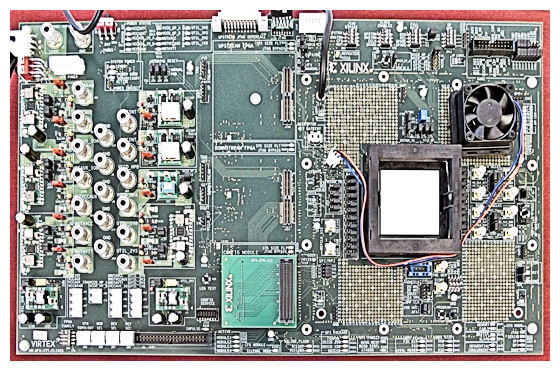
\includegraphics[height=60mm]{Figures/fpga.jpg}

% Title, author and degree
\vspace{0.8cm}
{\FontLb C Compiler for the VERSAT Reconfigurable Processor} \\
\vspace{3.6cm}
{\FontMb Gonçalo da Conceição Reis dos Santos} \\
\vspace{1.9cm}
{\FontLn Thesis to obtain the Master of Science Degree in} \\
\vspace{0.3cm}
{\FontLb Electrical and Computer Engineering} \\
%\vspace{1.9cm}
\vspace{1.0cm}
{\FontSn %
\begin{tabular}{ll}
Supervisor: & Prof. José João Henriques Teixeira de Sousa
\end{tabular} } \\
\vspace{1.0cm}
{\FontMb Examination Committee} \\
\vspace{0.3cm}
{\FontSn %
\begin{tabular}{ll}
Chairperson: & Prof. Francisco André Corrêa Alegria\\
Supervisor: & Prof. José João Henriques Teixeira de Sousa \\
Member of the Committee: & Prof. Paulo Ferreira Godinho Flores \\
\end{tabular} } \\
\vspace{1.5cm}
{\FontMb November 2019} \\
%
\end{center}

\cleardoublepage
 % file "Thesis_FrontCover.tex"
%\cleardoublepage

% ----------------------------------------------------------------------
% Dedication page (optional)
% ----------------------------------------------------------------------
%%%%%%%%%%%%%%%%%%%%%%%%%%%%%%%%%%%%%%%%%%%%%%%%%%%%%%%%%%%%%%%%%%%%%%%%%
%                                                                      %
%     File: Thesis_Dedication.tex                                      %
%     Tex Master: Thesis.tex                                           %
%                                                                      %
%     Author: Andre C. Marta                                           %
%     Last modified :  2 Jul 2015                                      %
%                                                                      %
%%%%%%%%%%%%%%%%%%%%%%%%%%%%%%%%%%%%%%%%%%%%%%%%%%%%%%%%%%%%%%%%%%%%%%%%

\null\vskip5cm%
\begin{flushright}
     Dedicated to someone special...
\end{flushright}
\vfill\newpage

 % file "Thesis_Dedication.tex"
%\cleardoublepage

% ----------------------------------------------------------------------
%  Acknowledgments (optional)
% ----------------------------------------------------------------------
%%%%%%%%%%%%%%%%%%%%%%%%%%%%%%%%%%%%%%%%%%%%%%%%%%%%%%%%%%%%%%%%%%%%%%%%%
%                                                                      %
%     File: Thesis_Acknowledgments.tex                                 %
%     Tex Master: Thesis.tex                                           %
%                                                                      %
%     Author: Andre C. Marta                                           %
%     Last modified :  2 Jul 2015                                      %
%                                                                      %
%%%%%%%%%%%%%%%%%%%%%%%%%%%%%%%%%%%%%%%%%%%%%%%%%%%%%%%%%%%%%%%%%%%%%%%%

\section*{\acknowledgments}

% Add entry in the table of contents as section
\addcontentsline{toc}{section}{\acknowledgments}

I want to thank my supervisor, Professor José Teixeira de Sousa, for the 
opportunity to develop this work and for his guidance and support during that process. 
His help was fundamental to overcome the multiple obstacles that I faced during this work.

I also want to acknowledge Professor Horácio Neto for providing a simple Convolutional 
Neural Network application, used as a basis for the application developed for the 
RV32-Versat architecture.

A special acknowledgement goes to my friends, for their continuous support, and Válter,  
that is developing a multi-layer architecture for RV32-Versat. When everything seemed to 
be doomed he always had a miraculous solution.

Finally, I want to express my sincere gratitude to my family for giving me all the 
support and encouragement that I needed throughout my years of study and through the 
process of researching and writing this thesis. They are also part of this work.\\

\textbf{Thank you.}

 % file "Thesis_Acknowledgements.tex"
%\cleardoublepage

% ----------------------------------------------------------------------
%  Abstract (both in English and Portuguese)
% ----------------------------------------------------------------------
%%%%%%%%%%%%%%%%%%%%%%%%%%%%%%%%%%%%%%%%%%%%%%%%%%%%%%%%%%%%%%%%%%%%%%%%%
%                                                                      %
%     File: Thesis_Resumo.tex                                          %
%     Tex Master: Thesis.tex                                           %
%                                                                      %
%     Author: Carlos A. Rodrigues                                           %
%     Last modified : 21 Jan 2011                                      %
%                                                                      %
%%%%%%%%%%%%%%%%%%%%%%%%%%%%%%%%%%%%%%%%%%%%%%%%%%%%%%%%%%%%%%%%%%%%%%%%

\section*{Resumo}

% Add entry in the table of contents as section
\addcontentsline{toc}{section}{Resumo}

Inserir o resumo em Portugu\^{e}s aqui com o máximo de 250 palavras e acompanhado de 4 a 6 palavras-chave...

\vfill

\textbf{\Large Palavras-chave:} OpenRISC, Sistema em um chip,...

\cleardoublepage

   % file "Thesis_Resumo.tex"
%\cleardoublepage

%%%%%%%%%%%%%%%%%%%%%%%%%%%%%%%%%%%%%%%%%%%%%%%%%%%%%%%%%%%%%%%%%%%%%%%%%
%                                                                      %
%     File: Thesis_Abstract.tex                                        %
%     Tex Master: Thesis.tex                                           %
%                                                                      %
%     Author: Andre C. Marta                                           %
%     Last modified :  2 Jul 2015                                      %
%                                                                      %
%%%%%%%%%%%%%%%%%%%%%%%%%%%%%%%%%%%%%%%%%%%%%%%%%%%%%%%%%%%%%%%%%%%%%%%%

\section*{Abstract}

% Add entry in the table of contents as section
\addcontentsline{toc}{section}{Abstract}

Versat is a Coarse-Grain Reconfigurable Array architecture (CGRA), which
implements self and partial reconfiguration by using a simple controller
unit. This report studies the current state of the art in HDL and CGRA
simulation, providing a basis to the development of a simulation environment for
Versat. The main objective of this environment is to provide a faster way to
develop and debug software without the use of prototyping hardware. Therefore,
the two types of HDL simulators, event-driven and cycle-accurate, their
advantages and disadvantages are studied, along with a performance comparison
between them. A study of high-level implementations for CGRA simulation is
also presented.

\vfill

\textbf{\Large Keywords:} Versat, coarse-grain reconfigurable arrays, HDL
simulation, CGRA simulation, high-level simulation

 % file "Thesis_Abstract.tex"
%\cleardoublepage

% ----------------------------------------------------------------------
%  Table of contents, list of tables, list of figures and nomenclature
% ----------------------------------------------------------------------

% Table of contents
%
\tableofcontents
%\cleardoublepage 

% List of tables
%
% Add entry in the table of contents as section
\phantomsection
%\addcontentsline{toc}{section}{\listtablename}
% Generate list
%\listoftables
%\cleardoublepage 

% List of figures
%
% Add entry in the table of contents as section
\phantomsection
%\addcontentsline{toc}{section}{\listfigurename}
% Generate list
%\listoffigures
%\cleardoublepage 

% Nomenclature
%
% entries of nomenclature list
%%%%%%%%%%%%%%%%%%%%%%%%%%%%%%%%%%%%%%%%%%%%%%%%%%%%%%%%%%%%%%%%%%%%%%%%%
%                                                                      %
%     File: Thesis_Nomenclature.tex                                    %
%     Tex Master: Thesis.tex                                           %
%                                                                      %
%     Author: Gonçalo Santos                                           %
%     Last modified : 20 Oct 2018                                      %
%                                                                      %
%%%%%%%%%%%%%%%%%%%%%%%%%%%%%%%%%%%%%%%%%%%%%%%%%%%%%%%%%%%%%%%%%%%%%%%%
%
% The definitions can be placed anywhere in the document body
% and their order is sorted by <symbol> automatically when
% calling makeindex in the makefile
%
% The \glossary command has the following syntax:
%
% \glossary{entry}
%
% The \nomenclature command has the following syntax:
%
% \nomenclature[<prefix>]{<symbol>}{<description>}
%
% where <prefix> is used for fine tuning the sort order,
% <symbol> is the symbol to be described, and <description> is
% the actual description.

% ----------------------------------------------------------------------
% Roman symbols [r]
\nomenclature[ru]{$\bf u$}{Velocity vector.}
\nomenclature[ru]{$u,v,w$}{Velocity Cartesian components.}
\nomenclature[rp]{$p$}{Pressure.}
\nomenclature[rC]{$C_D$}{Coefficient of drag.}
\nomenclature[rC]{$C_L$}{Coefficient of lift.}
\nomenclature[rC]{$C_M$}{Coefficient of moment.}

% ----------------------------------------------------------------------
% Greek symbols [g]
\nomenclature[g]{$\rho$}{Density.}
\nomenclature[g]{$\alpha$}{Angle of attack.}
\nomenclature[g]{$\beta$}{Angle of side-slip.}
\nomenclature[g]{$\mu$}{Molecular viscosity coefficient.}
\nomenclature[g]{$\kappa$}{Thermal conductivity coefficient.}

% ----------------------------------------------------------------------
% Subscripts [s]
\nomenclature[s]{$x,y,z$}{Cartesian components.}
\nomenclature[s]{$i,j,k$}{Computational indexes.}
\nomenclature[s]{$\infty$}{Free-stream condition.}
\nomenclature[s]{ref}{Reference condition.}
\nomenclature[s]{$n$}{Normal component.}

% ----------------------------------------------------------------------
% Supercripts [t]
\nomenclature[t]{T}{Transpose.}
\nomenclature[t]{*}{Adjoint.}

 % file "Thesis_Nomenclature.tex"
%
% Add entry in the table of contents as section
\phantomsection
%\addcontentsline{toc}{section}{\nomname}
% Insert glossary/nomenclature section produced by MakeIndex
\printnomenclature
%\cleardoublepage

% entries of glossary list
%%%%%%%%%%%%%%%%%%%%%%%%%%%%%%%%%%%%%%%%%%%%%%%%%%%%%%%%%%%%%%%%%%%%%%%%%
%                                                                      %
%     File: Thesis_Glossary.tex                                        %
%     Tex Master: Thesis.tex                                           %
%                                                                      %
%     Author: Carlos A. Rodrigues                                           %
%     Last modified : 30 Oct 2012                                      %
%                                                                      %
%%%%%%%%%%%%%%%%%%%%%%%%%%%%%%%%%%%%%%%%%%%%%%%%%%%%%%%%%%%%%%%%%%%%%%%%
%
% The definitions can be placed anywhere in the document body
% and their order is sorted by <symbol> automatically when
% calling makeindex in the makefile
%
% The \glossary command has the following syntax:
%
% \glossary{entry}
%
% The \nomenclature command has the following syntax:
%
% \nomenclature[<prefix>]{<symbol>}{<description>}
%
% where <prefix> is used for fine tuning the sort order,
% <symbol> is the symbol to be described, and <description> is
% the actual description.

% ----------------------------------------------------------------------

\glossary{name={\textbf{MDO}},description={Multi-Disciplinar Optimization is an engineering technique that uses optimization methods to solve design problems incorporating two or more disciplines.}}

\glossary{name={\textbf{CFD}},description={Computational Fluid Dynamics is a branch of fluid mechanics that uses numerical methods and algorithms to solve problems that involve fluid flows.}}

\glossary{name={\textbf{CSM}},description={Computational Structural Mechanics is a branch of structure mechanics that uses numerical methods and algorithms to perform the analysis of structures and its components.}}

 % file "Thesis_Glossary.tex"

% Add entry in the table of contents as section
\phantomsection
%\addcontentsline{toc}{section}{\glossaryname}
% Insert glossary section produced by MakeIndex
\printglossary
%\cleardoublepage
\newpage

% Set arabic numbering (1,2,...) after preface
%
\setcounter{page}{1}
\pagenumbering{arabic}

% ----------------------------------------------------------------------
%  Chapters
% ----------------------------------------------------------------------

%%%%%%%%%%%%%%%%%%%%%%%%%%%%%%%%%%%%%%%%%%%%%%%%%%%%%%%%%%%%%%%%%%%%%%%%
%                                                                      %
%     File: Thesis_Introduction.tex                                    %
%     Tex Master: Thesis.tex                                           %
%                                                                      %
%     Author: Andre C. Marta                                           %
%     Last modified :  2 Jul 2015                                      %
%                                                                      %
%%%%%%%%%%%%%%%%%%%%%%%%%%%%%%%%%%%%%%%%%%%%%%%%%%%%%%%%%%%%%%%%%%%%%%%%

\chapter{Introduction}
\label{chapter:introduction}




In this report, the problem of accelerating the execution of Deep Neural
Networks (DNNs) using Coarse GRained Reconfigurable Arrays (CGRAs) is studied,
with special emphasis on compiling a DNN description into code that runs on
CPU/CGRA system. The Deep Versat Architecture~\cite{valter:deepversat} CGRA will be used as an
implementation tool in this work.


%%%%%%%%%%%%%%%%%%%%%%%%%%%%%%%%%%%%%%%%%%%%%%%%%%%%%%%%%%%%%%%%%%%%%%%%
\section{Problem}
\label{section:problem}

Neural Networks have been an object of study since the 1940's, but until the
beginning of this decade their applications were limited and did not play a
major role in computer vision conferences. With its meteoric rise in research,
several solutions to accelerate this algorithm have appeared, from Field Programmable Gate Arrays (FPGA) to
Application Specific Integrated Circuits (ASIC) implementations.

Convolutional Neural Networks (CNNs) are a particular kind of DNN where the output
values of the neurons in one layer are convolved with a kernel to produce the
input values of the neurons of the next layer. This algorithm is compute bound,
that is, its performance depends on how fast it can do certain calculations, and
depend less on the memory access time. Namely the convolutional layers take
approximately 90$\%$ of the computation time.

The acceleration of these workloads is a matter of importance for today's
applications such as image processing for object recognition or simply to
enhance certain images. Other uses like instant translation and virtual
assistants are applications of neural networks and their acceleration is of
vital importance to bring them into Internet of Things.

A suitable circuit to accelerate DNNs in hardware is the CGRA. A CGRA is a
collection of Functional Units and memories with programmable interconnections
in order to form computational datapaths. A CGRA can be implemented in both
FPGAs and ASICs. CGRAs can be reconfigured much faster than FPGAs, as they have
much less configuration bits. If reconfiguration is done at runtime, CGRAs add
temporal scalability to the spacial scalability that characterize
FPGAs. Moreover, partial reconfiguration is much easier to do in CGRAs compared
to FPGAs which further speeds up reconfiguration time. Another advantage of
CGRAs is the fact that they can be programmed entirely in software, contrasting
with the large development time of customized Intellectual Property (IP) blocks.
The Coarse Grain Reconfigurable Arrays (CGRA) is a midway acceleration solution
between FPGAs, which are flexible but large, power hungry and difficult to
reprogram, and ASICs, which are fast but generally not programmable.

However, mapping a specific DNN to a CGRA requires knowledge of its
architecture, latencies and register configurations, which may become a lengthy
process, especially if the user wants to explore the design space for several
DNN configurations. An automatic compiler that can map a standard DNN
description into CPU/CGRA code would dramatically decrease time to market of its
users. Currently there are equivalent tools for CPUs and GPUs and
even for FPGAS.


%%%%%%%%%%%%%%%%%%%%%%%%%%%%%%%%%%%%%%%%%%%%%%%%%%%%%%%%%%%%%%%%%%%%%%%%
\section{Solution}
\label{section:solution}

The proposed solution is a compiler that takes a configuration file from a
neural network framework like Caffe or Darknet. This new tool inputs the
parameters of Deep Versat, such as the number of layers and functional units,
and produces the C code needed for the Versat runs. This code is run on the
RISC-V picorv32~\cite{picorv} CPU controller that has Deep Versat as a peripheral.

%%%%%%%%%%%%%%%%%%%%%%%%%%%%%%%%%%%%%%%%%%%%%%%%%%%%%%%%%%%%%%%%%%%%%%%%
%\section{Thesis Outline}
%\label{section:outline}

%Briefly explain the contents of the different chapters...

%%%%%%%%%%%%%%%%%%%%%%%%%%%%%%%%%%%%%%%%%%%%%%%%%
%\section{Author's Work}
%\label{section:authorwork}

%TO ADD----

%%%%%%%%%%%%%%%%%%%%%%%%%%%%%%%%%%%%%%%%%%%%%%%%%%
\section{Report Outline}
\label{reportoutline}

This report is composed of 4 more chapters. In the second chapter, the
state-of-the-art of neural networks and the difficulties accelerating them is
described. In the third chapter, the Deep Versat architecture and how to program
it is explained. In the fourth chapter, CNN compiler techniques are
explored. Finally, the last chapter contains the proposed solution and the plan
for its execution.


 % file "Thesis_Introduction.tex"
\cleardoublepage

\chapter{Deep Neural Networks}
\label{chapter:DNN}

This chapter introduces the concept of Deep Neural Networks (DNNs) and proceeds to Convolutional Neural Networks (CNNs), a common form of DNN widely used in image processing applications such as object detection. The evolution of CNNs and the associated popular models are further discussed. Field Programmable Gate Arrays (FPGAs) have recently been used to accelerate CNNs by developing dedicated hardware and memory systems. Thus, this chapter also focuses on the strategies implemented in previous works to accelerate CNNs in FPGAs.

%%%%%%%%%%%%%%%%%%%%%%%%%%%%%%%%%%%%%%%%%%%%%%%%%%%%%%%%%%%%%%%%%%%%%%%%
\section{Neural networks}
\label{section:NNs}

The neuron is the main computational unit of neural networks and is implemented as the weighted sum of the inputs plus a constant, followed by an activation function, as represented in Fig.~\ref{fig:neuron}.

\begin{figure}[!htb]
  \centering
  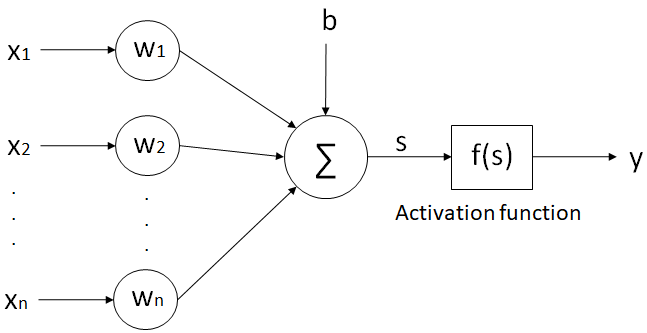
\includegraphics[width=0.45\textwidth]{Figures/neuron.png}
  \caption{Implementation of a neuron.}
  \label{fig:neuron}
\end{figure}
%\vspace{-2mm}

The weight, $w_{i}$, expresses the influence of a given input, $x_{i}$, to the neuron's output and the bias, $b$, is an offset term used to shift the result of the activation function, $f$, towards the negative or positive side. Eq. \ref{eq:NN} computes the output, $y$, of a neuron.

\begin{equation}
  y = f \left( b + \sum_{i=1}^{n} x_{i} w_{i} \right)
\label{eq:NN}
\end{equation}

Conventional activation functions include the identity function, the sigmoid (i.e., logistic function) and the hyperbolic tangent. Recently, the Rectified Linear Unit (ReLU) and some variations (e.g., Leaky ReLU) have become popular due to their simplicity and fast convergence during training~\cite{sze:dnn_survey}. These activation functions are represented in Fig.~\ref{fig:act_func}.    

\begin{figure}[!htb]
  \centering
  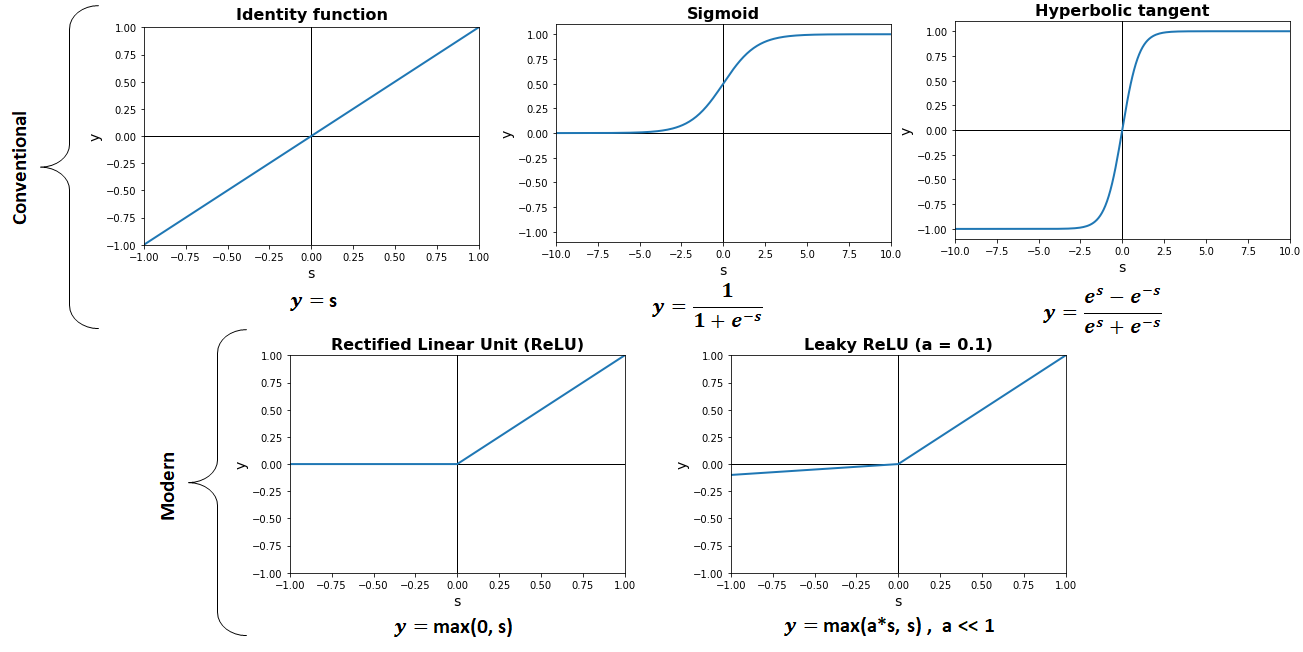
\includegraphics[width=\textwidth]{Figures/act_functions.png}
  \caption{Plot and expression of the most common activation functions.}
  \label{fig:act_func}
\end{figure}

Neural networks are composed by neurons organized in layers: one input layer, one or more hidden layers and one output layer. A DNN is a neural network with more than one hidden layer. Fig.~\ref{fig:DNN} exemplifies a fully connected (i.e., each neuron from one layer is connected to every neuron of the next layer) DNN with 2 hidden layers.

\vspace{-0.4cm}
\begin{figure}[!htb]
  \centering
  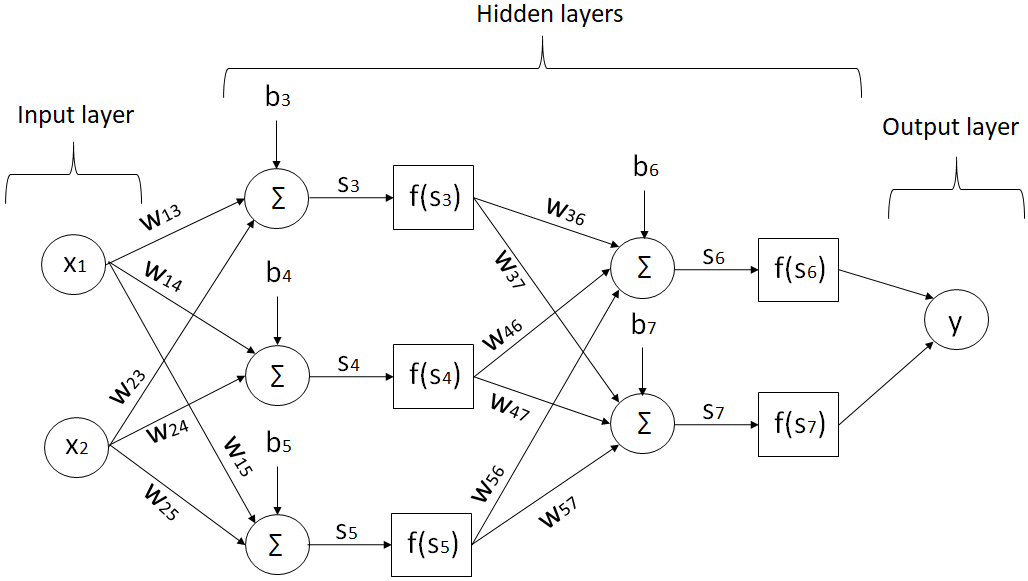
\includegraphics[width=0.7\textwidth]{Figures/DNN.png}
  \caption{Example of a fully connected DNN.}
  \label{fig:DNN}
\end{figure}

By using more layers, DNNs can learn more complex high-level features. For instance, in a typical image processing application, the input layer receives the normalized pixels (i.e., scaled between 0 and 1) from an image which then go through the first hidden layer. This layer outputs several low-level features (e.g., lines and edges). In the next hidden layers, these features are combined to form higher level features (e.g., contours, shapes). Hence, each layer builds on the features detected in previous layers. The output layer predicts if all those features describe a certain object or scene~\cite{sze:dnn_survey}. This process is an example of \textbf{inference}, which consists in making predictions over the input data by using a learned model. This work focuses on the inference for embedded systems, thus, a pre-trained DNN is used.

%%%%%%%%%%%%%%%%%%%%%%%%%%%%%%%%%%%%%%%%%%%%%%%%%%%%%%%%%%%%%%%%%%%%%%%%
\section{Convolutional Neural Networks}
\label{section:CNN}

Fully connected DNNs are more difficult to train as the network gets deeper due to the increasing number of connections and weights. CNNs are DNNs characterized by the presence of convolutional layers. The neurons of a convolutional layer only connect to sub-regions of the previous layer, instead of being fully connected, allowing to build deeper networks and therefore achieve superior performance. 

CNNs are implemented as a sequence of interconnected layers and consist in two stages: feature extraction and classification, as shown in Fig.~\ref{fig:CNN}. The stages are based on convolutional, pooling and fully connected layers. For feature extraction, the network is built on repeated blocks, each composed by a convolutional layer, an optional batch-normalization layer, a non-linear layer (i.e., application of an activation function) and an optional pooling layer. For classification purposes, fully connected layers, optionally followed by a regression function, are typically applied after the last block of the feature extraction stage. Modern CNN models add other type of layers such as shortcut, route and upsample layers. 

\begin{figure}[!htb]
  \centering
  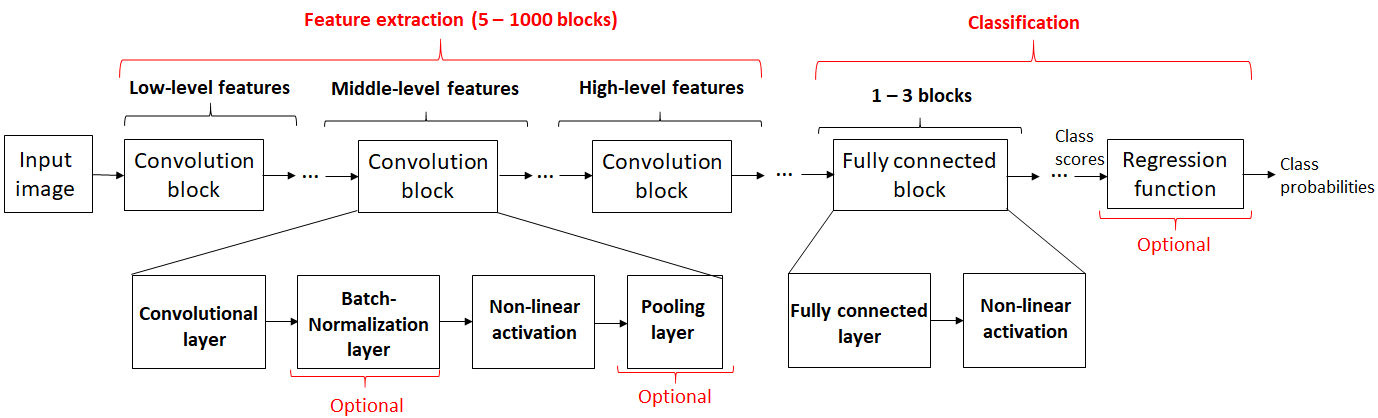
\includegraphics[width=\textwidth]{Figures/CNN.png}
  \caption{Constitution of a typical CNN.}
  \label{fig:CNN}
\end{figure}
\vspace{-6.5mm}

\subsection{Convolutional layer}

Convolutional layers perform 3D convolutions, which can be seen as a set of 2D convolutions. In 2D convolutions, a 2D kernel is overlapped and shifted as a sliding window throughout the entire 2D input image (known as input feature map), generating a 2D output image (called output feature map). In each overlap, a multiply and accumulate (MAC) operation is performed. Padding, which consists in adding new elements around the edges of the input feature map (FM), allows the output to keep the same size as the input. Normally zero-padding is applied. Fig.~\ref{fig:2D_conv} exemplifies a 2D convolution between an 5x5 input feature map and 3x3 kernel with zero padding. Note how the weights that compose the kernel are shared during the process. In this example, the step size (also known as stride) used when shifting the kernel throughout the input feature map is 1.   

\begin{figure}[!htb]
  \centering
  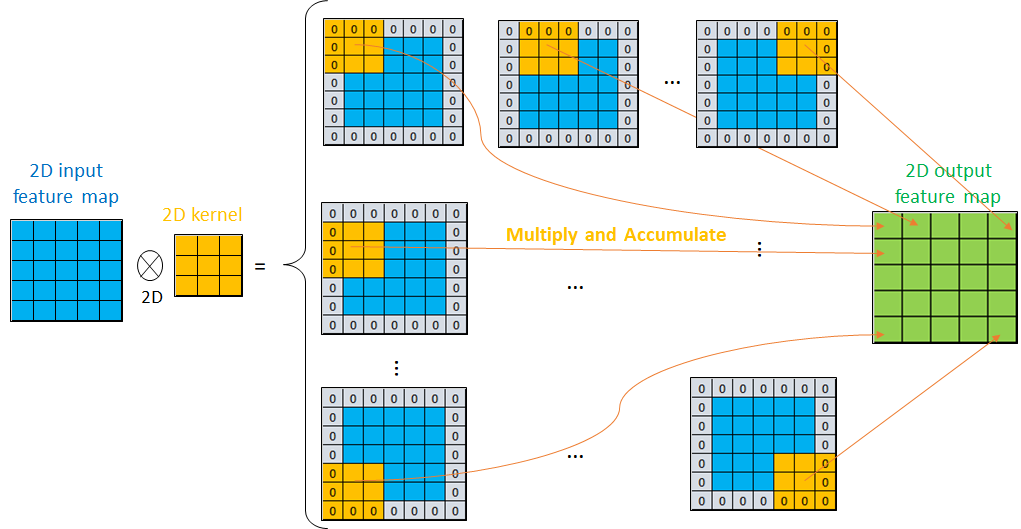
\includegraphics[width=0.9\textwidth]{Figures/2D_conv.png}
  \caption{Example of an 5x5 input feature map and 3x3 kernel 2D convolution.}
  \label{fig:2D_conv}
\end{figure}

The input of convolutional layers is a set of 2D feature maps (each one is called a channel) and another set of 3D kernels, with each 3D kernel having the same number of 2D channels. For each 3D kernel, there is a 2D convolution between each channel of the input feature map and each channel of the given 3D kernel. The results of the convolutions are summed across all the channels. The output feature map is obtained after summing the former result with a shared bias associated to each 3D kernel. Therefore, one output feature map is created for each 3D kernel. Fig.~\ref{fig:3D_conv} exemplifies a 3D convolution between an 5x5 input feature map and two 3x3 kernels, all with 3 channels and zero-padding.

\begin{figure}[!htb]
  \centering
  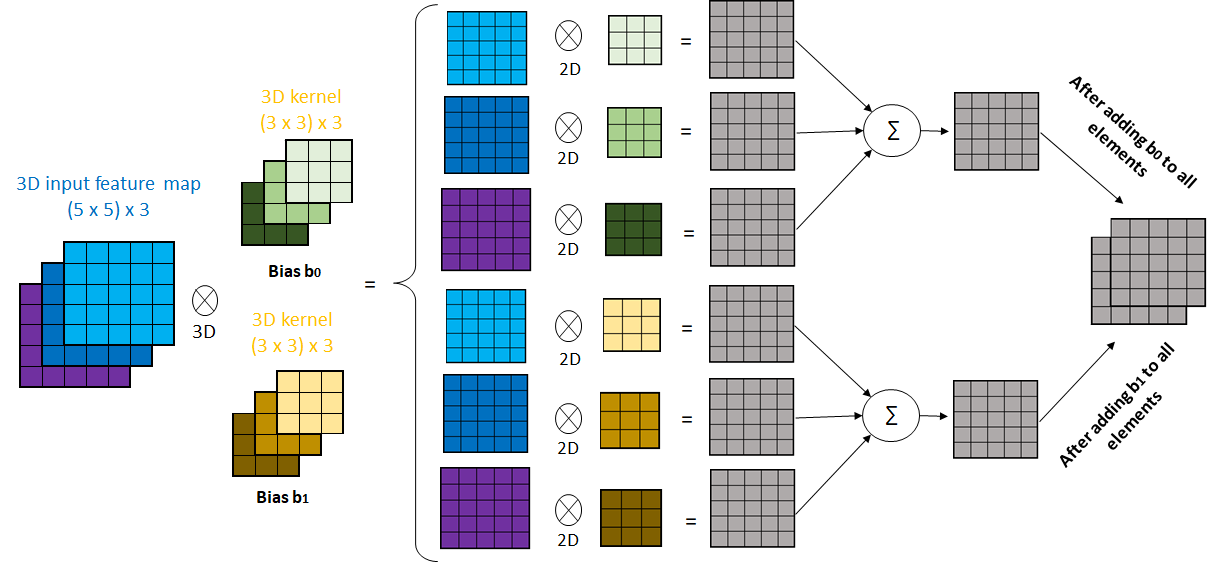
\includegraphics[width=\textwidth]{Figures/3D_conv.png}
  \caption{Example of an 5x5 input feature map and two 3x3 kernels 3D convolution (3 channels).}
  \label{fig:3D_conv}
\end{figure}
\vspace{-5mm}

\subsection{Batch-Normalization layer}

The batch-normalization layer is used for speeding up the training by normalizing the input data (i.e., zero mean and unit standard deviation)~\cite{Abdelouahab:dnn_survey}. Furthermore, the normalized value is scaled and shifted. Eq. \ref{eq:batch_norm} expresses the computation performed by this layer for each input element, $x$, where the mean, $\mu$, and the variance, $\sigma^2$, are statistics collected from training and the scale factor, $\gamma$, and the shift factor, $\beta$, are parameters learned during training. $\epsilon$ is a small constant that avoids dividing by zero. When using this layer, the bias can be included in the shift factor instead of being computed in the convolutional layer.

\begin{equation}
  y = \frac{x-\mu}{\sqrt{\sigma^2+\epsilon}} \gamma + \beta
\label{eq:batch_norm}
\end{equation}

In inference, the values of $\mu$, $\sigma^2$, $\gamma$ and $\beta$ are known. Thus, Eq. \ref{eq:batch_norm} can be reformulated as one multiplication and one addition, as shown in Eq. \ref{eq:batch_norm2}, where $\gamma_i$ and $\beta_i$ are the new scale and shift factors.

\begin{equation}
  y = x \times \frac{\gamma}{\sqrt{\sigma^2+\epsilon}} + \left( - \frac{\mu \times \gamma}{\sqrt{\sigma^2+\epsilon}} + \beta \right) = x \times \gamma_i + \beta_i
\label{eq:batch_norm2}
\end{equation}

\subsection{Pooling layer}

The pooling layer downsamples the feature maps, leading to a reduction of the number of parameters in the next layers. Each 2D channel is divided into non-overlapping blocks, which are further replaced by the maximum (max-pooling) or the mean (average pooling) value of the block. The most common operation is a 2x2 max-pooling, as shown in Fig.~\ref{fig:maxpool}. Some CNNs, instead of using pooling layers, simply apply a stride of 2 in the convolutional layers. However, pooling layers are more robust as they turn the network invariant to small shifts and distortions when downsampling~\cite{sze:dnn_survey}. 

\begin{figure}[!htb]
  \centering
  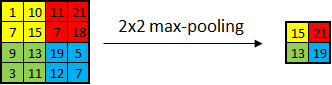
\includegraphics[width=0.45\textwidth]{Figures/maxpool.png}
  \caption{Example of 2x2 max-pooling.}
  \label{fig:maxpool}
\end{figure}
\vspace{-0.3cm}

\subsection{Shortcut layer}
The shortcut layer skips one or more layers by adding the output of a former layer to the input of the current layer. Fig.~\ref{fig:shortcut} exemplifies a shortcut layer generated from adding the output from 2 layers before.

\begin{figure}[!htb]
  \centering
  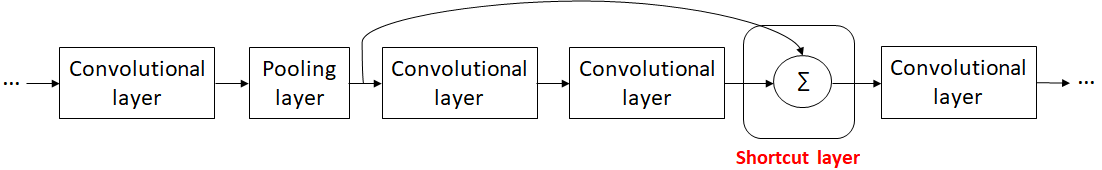
\includegraphics[width=0.85\textwidth]{Figures/shortcut_layer.png}
  \caption{Example of a shortcut layer.}
  \label{fig:shortcut}
\end{figure}
\vspace{-0.3cm}

\subsection{Route and upsample layers}

Route and upsample layers were introduced for CNNs focused on object detection tasks~\cite{Redmon2018YOLOv3AI}. The route layer concatenates the output from a former layer with the input of the current layer by stacking them into different channels. For example, routing a (26x26)x256 feature map with a (26x26)x128 feature map results in a (26x26)x384 feature map. This allows the detection of fine grained features, improving the localization of small objects. 

The upsample layer upsamples a feature map, typically by a factor of two, which allows to detect objects at different scales and obtain more meaningful semantic information from the features. Fig.~\ref{fig:upsample} exemplifies the simplest way to upsample a 2x2 feature map by a factor of two. 

\begin{figure}[!htb]
  \centering
  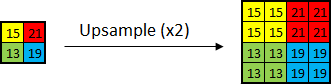
\includegraphics[width=0.45\textwidth]{Figures/upsample.png}
  \caption{Example of upsampling by a factor of 2.}
  \label{fig:upsample}
\end{figure}
\vspace{-0.4cm}

%%%%%%%%%%%%%%%%%%%%%%%%%%%%%%%%%%%%%%%%%%%%%%%%%%%%%%%%%%%%%%%%%%%%%%%%
\section{Training neural networks}
\label{section:training}

The training of neural networks consists in finding the parameters (i.e., weights and bias) that maximize the score of the correct prediction and minimize the scores of the incorrect predictions. For that, there is a training dataset containing inputs of the network (e.g., an image) and the desired output (e.g., label). In order to obtain the parameters, the gradient descent method~\cite{sze:dnn_survey} is used. This iterative algorithm updates the parameters by computing the partial derivatives of the gradient, which indicates how the parameters should change to reduce the difference between the desired outputs and the actual predictions (also known as loss). To efficiently compute the partial derivatives, the loss is propagated backwards through the network, which is known as the backpropagation algorithm~\cite{sze:dnn_survey}.  

Often, the parameters are initialized randomly for the first iteration of the gradient descent, which could result in slow training. To speed-up the training and achieve better performance, fine-tuning can be applied. Fine-tuning consists in using previously-trained parameters as a starting point to adjust the data to a new dataset or a new constraint.

There are several frameworks for training and testing DNN models. The most popular are Caffe, Tensorflow, Torch~\cite{sze:dnn_survey} and Darknet~\cite{Redmon2015YouOL}. The popular CNN models that will be mentioned in the next section were developed for image classification. The most popular datasets for this task are MNIST (digit classification), CIFAR and ImageNet~\cite{sze:dnn_survey}.

%%%%%%%%%%%%%%%%%%%%%%%%%%%%%%%%%%%%%%%%%%%%%%%%%%%%%%%%%%%%%%%%%%%%%%%%

\section{Popular CNN models}
\label{section:popular_models}

AlexNet~\cite{sze:dnn_survey} was one of the first CNN-based models for image classification, followed by VGG-16~\cite{sze:dnn_survey}. Both are based on the architecture presented in Fig.~\ref{fig:CNN}. They mainly differ in the number of layers and in the number and size of the kernels. A more distinct model is GoogLeNet~\cite{sze:dnn_survey}. Different sized filters are convoluted in parallel for the same input feature map and the results are further concatenated. Therefore, the input is processed at multiple scales. The other difference is the use of 1x1 kernels to reduce the number of channels and, consequently, the number of weights. 

ResNet~\cite{sze:dnn_survey} was the first CNN that exceeded the human-level accuracy for image classification by deploying a deeper network than the above-mentioned models. Those models suffered from the vanishing gradient problem, restraining them from getting deeper. When training, after several multiplications, the gradient becomes infinitely small during backpropagation, affecting the update of the weights in early layers for very deep networks. To avoid that, shortcut layers were added in the network.

Darknet-53~\cite{Redmon2018YOLOv3AI} is a more recent CNN model that also employs the shorcut layers first introduced by ResNet to allow a deeper network.  

%%%%%%%%%%%%%%%%%%%%%%%%%%%%%%%%%%%%%%%%%%%%%%%%%%%%%%%%%%%%%%%%%%%%%%%%
\section{FPGA-based CNNs}
\label{section:fpga_cnn}

Several studies have been conducted for accelerating CNNs in FPGAs~\citep{ma:loop_opt, sze:dnn_survey, Abdelouahab:dnn_survey, Guo:dnn_survey}. The main computation in CNNs is the MAC operation which mostly occurs in the convolutional layers, as shown in Table~\ref{tab:DNN}. Consequently, more than 90\% of the inference execution time is typically spent in the computation of the convolutional layers~\cite{Abdelouahab:dnn_survey}. Therefore, accelerators are focused on speeding-up these layers.

\vspace{+0.1cm}
\begin{table}[!htb]
    \footnotesize
    \centering
    \caption{Layer constitution of some popular DNN models (adapted from~\cite{Abdelouahab:dnn_survey}).}
    \label{tab:DNN}
    \begin{tabular}{|c|c|c|c|c|c|}
    \hline
            Type of layer              &  Characteristic & AlexNet &   VGG-16   &  GoogLeNet  &    ResNet-152  \\ \hline
   {\multirow{3}{*}{{Convolutional}}}  &     \# Layers   &    5    &    13     &      57     &     155    \\ \cline{2-6}
                                       &     \# MACs     &   666M  &   15.3G   &    1.58G    &    11.3G   \\ \cline{2-6} 
                                       &  \#Parameters   &  2.33M  &   14.7M   &    5.97M    &     58M    \\ \hline
              Pooling                  &      \# Layers   &    3    &    5     &      14     &      2     \\ \hline 
  {\multirow{3}{*}{{Fully Connected}}} &     \# Layers   &     3    &    3     &      1      &      1     \\ \cline{2-6}
                                       &     \# MACs     &   58.6M  &   124M   &    1.02M    &    2.05M   \\ \cline{2-6} 
                                       &  \#Parameters   &   58.6M  &   124M   &    1.02M    &    2.05M   \\ \hline
    \end{tabular}
\end{table}

The most common approaches for accelerating CNN inference in FPGAs in previous works are mainly focused on optimizing the accelerator by developing dedicated hardware and memory systems in order to exploit the parallelism of the MAC operations and to enhance data reuse. Approximating the model specifically for computation in FPGAs is another method that allows to reduce the amount of operations and storage requirements.

\subsection{Accelerator optimization}
\label{subsection:acc_opt}

One of the main advantages of accelerating CNNs in FPGAs, rather than in CPUs or GPUs, is the flexibility to design costumed hardware to exploit different sources of parallelism and dedicated caches to support data reuse. As shown in Table~\ref{tab:DNN}, as networks get deeper, the number of operations and the storage requirements increase. Consequently, the use of external memory is required, whose access results in high latency and significant energy consumption. FPGAs present a density of hard-wired Digital Signal Processing (DSP) blocks and a collection of on-chip memories that can be used for performing the MAC operations and reducing the number of external memory accesses, respectively.

Typical FPGA-based CNN accelerators~\cite{qiu:fpga_acc, zhang:fpga_acc, suda:fpga_acc} introduce several levels of memory hierarchy, as shown in Fig.~\ref{fig:fpga_cnn}. The system is composed by two on-chip input buffers, one for fetching the feature maps and the other for fetching the parameters (i.e., weights and bias) from the external memory through the DMA. The data is streamed into configurable processing elements (PEs), which are responsible for computing the MAC operations. Each PE has its own on-chip registers. The on-chip output buffer stores the intermediate results and output feature maps, which are transferred back, if needed, to the external memory. The CPU issues the workload to the controller, which in turn generates control signals to the other modules. The multipliers and adder trees present in each PE are usually pipelined in order to reduce the critical path of the circuit and increase the throughput.

\begin{figure}[!htb]
  \centering
  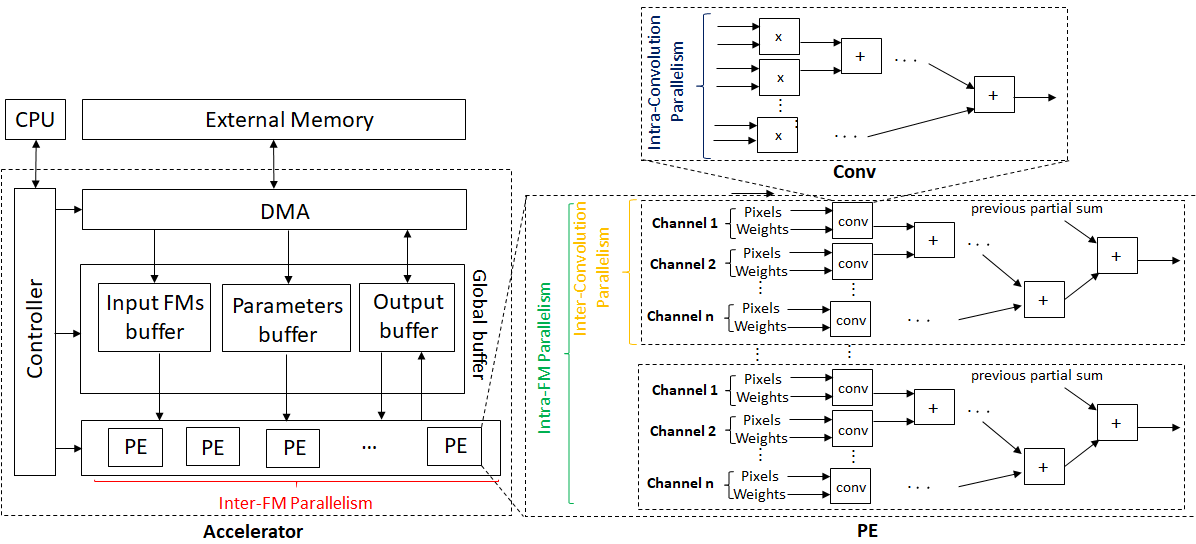
\includegraphics[width=\textwidth]{Figures/fpga_cnn.png}
  \caption{Typical FPGA-based CNN accelerator (adapted from~\cite{Abdelouahab:dnn_survey}).}
  \label{fig:fpga_cnn}
\end{figure}

Fig.~\ref{fig:fpga_cnn} also shows four sources of concurrency~\cite{Abdelouahab:dnn_survey} when computing each convolutional layer:\\
1) \underline{Intra-Convolution Parallelism:} multiplications in 2D convolutions are implemented concurrently.\\
2) \underline{Inter-Convolution Parallelism:} multiple 2D convolutions are computed concurrently.\\
3) \underline{Intra-FM Parallelism:} multiple pixels of a single output FM are processed concurrently.\\
4) \underline{Inter-FM Parallelism:} each output FM is processed separately in a different PE.

The computation of each convolutional layer can be seen as the application of four nested loops. Each loop is associated to a source of parallelism, as represented in Fig.~\ref{fig:loop_parall}.

\begin{figure}[!htb]
  \centering
  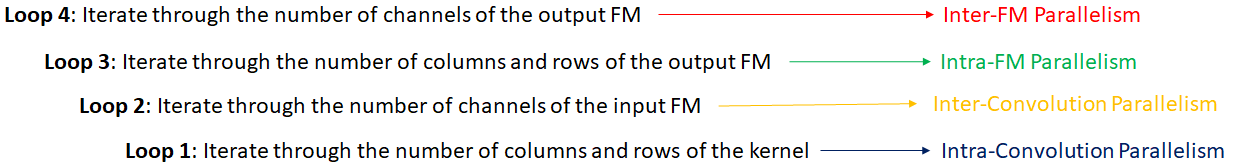
\includegraphics[width=\textwidth]{Figures/loop_parall.png}
  \caption{Association between loops and source of parallelism.}
  \label{fig:loop_parall}
\end{figure}

The sources of parallelism to be exploited depend on the characteristics of the convolutional layers (e.g., number of channels, input feature map size) and the FPGA resources. The architectural configuration of the PEs (i.e., number of MACs and registers) and the data temporal scheduling are defined by applying loop optimization techniques such as loop unrolling, loop tiling and loop interchange~\cite{Abdelouahab:dnn_survey}. Examples of previous works that implement these techniques are analyzed in section \ref{subsection:comparison_fpga_acc}.\\

\vspace{-0.5cm}

\textbf{Loop unrolling} consists in accelerating the execution of the loops at the expense of resource utilization. Each loop has an unroll factor that indicates how many times the respective loop is parallelized. Taking into account the loop enumeration in Fig.~\ref{fig:loop_parall}, the unroll factor for loop 4 determines the number of PEs while the unroll factors for the remaining loops determine the number of multipliers, adders and registers of each PE. The total number of multipliers is given by the product of the four unroll factors. The unroll factors must be carefully chosen, otherwise, they could lead to underutilization of the hardware. For instance, for any given loop, if the number of iterations is not divisible by the respective unrolling factor, then, the utilization ratio is less than 1~\cite{Guo:dnn_survey}. Fig.~\ref{fig:unroll_reuse} shows that the weights and the pixels can be reused by unrolling loops 3 and 4 respectively~\cite{ma:loop_opt}.

\vspace{-0.2cm}
\begin{figure}[!htb]
  \centering
  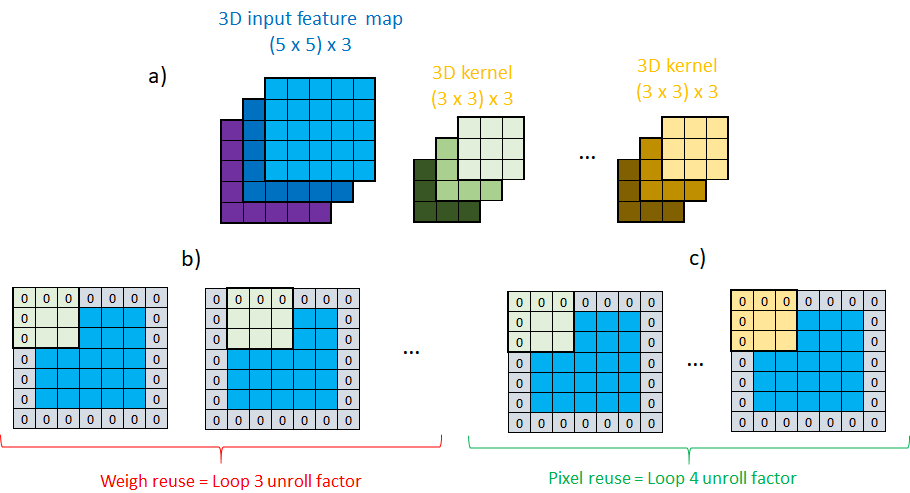
\includegraphics[width=0.85\textwidth]{Figures/unroll_reuse.png}
  \caption{a) 3D convolution between one FM and several kernels with b) weight and c) pixel reuse.}
  \label{fig:unroll_reuse}
\end{figure}

\textbf{Loop tiling} is a higher level of loop unrolling that divides the data into multiple blocks that fit into the on-chip buffers, increasing the data locality. Each tiled loop is splitted into two loops: one for iterating inside each tile (intra-tiling) and the other for iterating over the tiles (inter-tiling). Each loop has a tiling factor that indicates how many iterations are performed inside the respective tile. The tiling factors determine the size of the input and output buffers. If the tiling factors can cover all pixels and weights for loops 1 and 2, the partial sums (between channels) are stored in the local registers~\cite{ma:loop_opt}. Otherwise, the partial sums of one tile must be stored in the output buffer (intermediate result) until is used by the next tile~\cite{ma:loop_opt}. Fig.~\ref{fig:loop_tiling} exemplifies the division of the feature maps and kernels when tiling all loops.

\vspace{-0.2cm}
\begin{figure}[!htb]
  \centering
  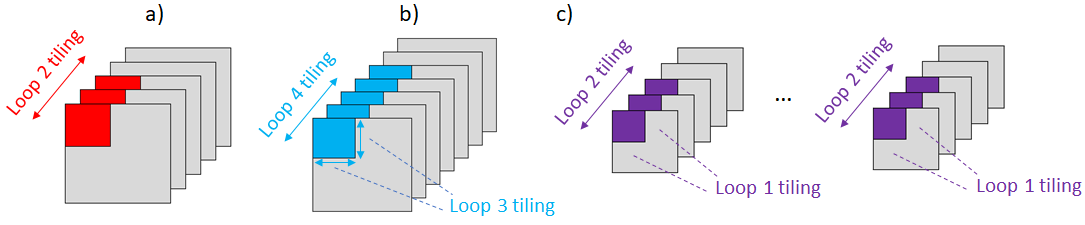
\includegraphics[width=0.85\textwidth]{Figures/loop_tiling.png}
  \caption{Example of loop tiling in the a) input FMs, b) output FMs and c) kernels.}
  \label{fig:loop_tiling}
\end{figure}
%\vspace{-0.5cm}

The \textbf{loop interchange} strategy decides the execution order of the loops. For intra-tiling loops, the order determines the data being transferred from the on-chip buffers to the PEs. For inter-tiling loops, the order indicates the movement of data from the external memory to the on-chip buffers. The storage required for intermediate results also depends on the order of the execution of the loops. For instance, the earlier loops 1 and 2 are computed, the fewer are the number of partial sums~\cite{ma:loop_opt}. 

\subsection{Model approximation}

The CNN execution can be accelerated by approximating the computation at the cost of minimal accuracy drop. Two of the most common strategies are reducing the precision and the number of operations. During training, the data is typically in single-precision floating-point format (32 bits). For inference in FPGAs, the feature maps and kernels can be converted to fixed-point format with less precision (typically 8 or 16 bits), reducing the storage requirements, hardware utilization and power consumption~\cite{Abdelouahab:dnn_survey}. 

The reduction of the FPGA resources consumption when using fixed-point representation is clear in Table~\ref{tab:resource_cons}, especially for lower precision data. The DSP consumption is hardly benefited when using narrower bit-width than 16 for fixed-point. Fig.~\ref{fig:fp_conv} exemplifies the conversion of a 32-bit floating-point value to fixed-point with 8 bits for the decimal part and 8 bits for the fractional part (Q8.8).

\vspace{+0.1cm}
\begin{table}[!htb]
    \footnotesize
    \centering
    \caption{Operation resource consumption for different operand sizes (adapted from~\cite{Guo:dnn_survey}).}
    \label{tab:resource_cons}
    \begin{tabular}{|c|c c|c c|c c c|}
    \hline
   \multirow{2}{*}{Data type} & \multicolumn{2}{|c|}{Multiplier} & \multicolumn{2}{|c|}{Adder} & \multicolumn{3}{|c|}{Multiplier and Adder} \\ \cline{2-8}
                              & LUT & FF & LUT & FF & LUT & FF & DSP \\ \hline
   floating-point (32 bits)   & 708 & 858 & 430 & 749 & 800 & 1284 & 2 \\ \hline
   floating-point (16 bits)   & 221 & 303 & 211 & 337 & 451 & 686 & 1 \\ \hline
   fixed-point (32 bits)      & 1112 & 1143 & 32 & 32 & 111 & 64 & 4  \\ \hline
   fixed-point (16 bits)      & 289 & 301 & 16 & 16 & 0 & 0 & 1  \\ \hline
   fixed-point (8 bits)       & 75 & 80 & 8 & 8 & 0 & 0 & 1  \\ \hline
   fixed-point (4 bits)       & 17 & 20 & 4 & 4 & 0 & 0 & 1  \\ \hline
    \end{tabular}
\end{table}

\vspace{-0.5cm}
\begin{figure}[!htb]
  \centering
  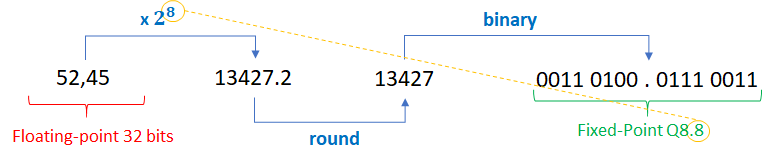
\includegraphics[width=0.7\textwidth]{Figures/fp_conv.png}
  \caption{Example of conversion from 32 bits floating-point to Q8.8 fixed-point.}
  \label{fig:fp_conv}
\end{figure}

In general, the feature maps of deeper layers tend to present a larger numerical range than the ones from initial layers and the weights also tend to be much smaller than the feature maps~\cite{Guo:dnn_survey}. Moreover, to prevent overflow, the precision must be increased for intermediate results. Thus, different precision values are normally used for weights, intermediate results and output feature maps from different layers. 

In order to reduce the number of operations, the most common approaches are weight pruning and low rank approximation~\cite{Abdelouahab:dnn_survey}. These methods are often followed by a fine-tuning phase to counterbalance the accuracy drop. As this work is focused on the inference part, these methods are not further studied.

\subsection{Comparison of FPGA-based CNN accelerators}
\label{subsection:comparison_fpga_acc}

To choose the unroll and tiling factors that maximize both computational throughput and resource utilization, besides minimizing the number of memory accesses, previous works performed a brute force exploration of the design space~\cite{Abdelouahab:dnn_survey}. This design space exploration consists in testing several factors for different loops in order to exploit various parallelism and data reuse patterns.

~\cite{zhang:fpga_acc} was one of the first works to employ loop optimization strategies to accelerate the execution of AlexNet in a FPGA. By unrolling loops 2 and 4, the accelerator achieved a computational throughput of 61.62 GOPs, relying on 32-bit floating point arithmetic. This work also introduced the utilization of double buffers to perform ping-pong operations, allowing to simultaneously compute and transfer data.

Greater acceleration can be achieved when using loop optimization techniques alongside fixed-point arithmetic. For instance,~\cite{suda:fpga_acc} reached a computational throughput of 187.24 GOPs for the same AlexNet network by unrolling loops 1, 2 and 4, relying on 16-bit fixed-point arithmetic. In general, unrolling loop 1 does not provide enough parallelism as the kernels are usually small (e.g. 3x3). Unrolling loop 1 also increases control complexity when layers present different kernel sizes. 
 
The same unrolling scheme and fixed point arithmetic was followed by~\cite{qiu:fpga_acc} for the VGG-16 network, achieving a throughput of 136.97 GOPs. In all these approaches, the loops are unrolled in the same way they are tilled~\cite{Abdelouahab:dnn_survey}. In~\cite{ma:loop_opt}, the tiling factors are set in a way all the data required to compute an element from the output feature map is fully buffered. As a result, intermediate results can be stored in the PE registers instead of in the output buffer. This accelerator outperforms all previous implementations by reusing pixels and weights when unrolling loops 3 and 4, reaching a total throughput of 645.25 GOPs.  

Table~\ref{tab:comp_fpga_acc} compares the four FPGA-based accelerators in terms of resource consumption, optimization strategy and throughput. All these approaches unroll loop 4 by employing several PEs.~\cite{zhang:fpga_acc} has the major DSP consumption mainly due to using 32-bit floating point operands.~\cite{ma:loop_opt} presents 3 times higher throughput than~\cite{qiu:fpga_acc} but consumes the double of resources in terms of DSPs and on-chip memory (BRAMs). The analysis of previous works regarding FPGA-based CNN acceleration allows to infer that a design exploration is essential for achieving optimal unroll and tiling factors, which in turn depend on the characteristics of the convolutional layers and the available resources of the FPGA. 

\vspace{+0.1cm}
\begin{table}[!htb]
    \footnotesize
    \centering
    \caption{Comparison between different FPGA-based accelerators.}
    \label{tab:comp_fpga_acc}
    \begin{tabular}{|>{\columncolor[gray]{0.8}}c|c|c|c|c|}
    \hline
    Network & AlexNet~\cite{zhang:fpga_acc} & AlexNet~\cite{suda:fpga_acc} & VGG-16~\cite{qiu:fpga_acc} & VGG-16~\cite{ma:loop_opt} \\ \hline
    Device & Virtex VX485T & Stratix5 GSD8 & Zynq XC7Z045 & Arria-10 GX 1150  \\ \hline
    Frequency (MHz) & 100 & 120 & 150 & 150 \\ \hline
    \# Operations (GOP) & 1.3 & 1.3 & 30.76 & 30.95\\ \hline
    \# Weights (M) & 2.3 & 2.3 & 50.18 & 138.3\\ \hline
    LUT (K) & 186 & 138 & 183 & 161\\ \hline
    BRAM & 512 (36 kB) & --- &  486 (36 kB) & 1900 (20 kB) \\ \hline
    DSP & 2240 & 635 & 780 & 1518 \\ \hline
    Throughput (GOPs) & 61.62 & 126.6 & 136.97 & 645.25 \\ \hline
    Unrolled loops & 2,4 & 1,2,4 & 1,2,4 & 3,4 \\ \hline
    Precision & Float 32 & Fixed 16 & Fixed 16 & Fixed 8-16\\ \hline
    \end{tabular}
\end{table}

\subsubsection{Final remarks}

CNNs are composed by a sequence of interconnected layers, being the convolutional ones the most time consuming for inference execution. FPGAs, with dedicated hardware and cache memories, allows to exploit parallelism and data reuse. Previous works use fixed-point arithmetic and perform design space exploration to obtain the best loop optimization parameters. A similar study will need to be conducted to accelerate the convolutional layers of the object detection network chosen in the next chapter. % file "Thesis_DNN.tex"
\chapter{Object Detection State-of-Art}
\label{chapter:object_detection}

This chapter studies the current CNN-based state-of-art object detectors, alongside the benchmarks and metrics used for their evaluation. Based on this study, one object detector is chosen and described.\\

\vspace{-0.4cm}
The task of a general-purpose object detector is to locate and classify existing objects in an image from predefined categories. The most common way to label and output the coordinates of the located object is to draw a bounding box around it, as represented in Fig.~\ref{fig:bounding_box}. State-of-art object detectors are DNN-based and their backbone network for feature extraction consists (or is inspired) in the networks for image classification mentioned in the section \ref{section:popular_models}, excluding the last fully connected layers~\cite{jiao:obj_survey}.   

\begin{figure}[!htb]
  \centering
  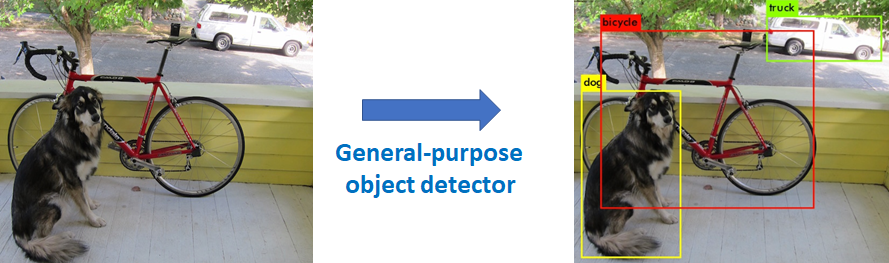
\includegraphics[width=0.7\textwidth]{Figures/bounding_box.png}
  \caption{Example of bounding box usage to locate objects in an image (adapted from~\cite{Redmon2015YouOL}).}
  \label{fig:bounding_box}
\end{figure}
\vspace{-0.2cm}

\section{Benchmarks and metrics}
\label{section:benchmarks}

Two of the most common benchmarks for general-purpose object detection are PASCAL VOC 2007/2012 and Microsoft COCO~\cite{zhao:obj_survey}. The official metric for measuring the performance of detectors is based on the mean average precision (mAP) with small variations between both benchmarks. This metric compares the predicted bounding boxes and labels with the ground truth data, which provides the true labels of each object in an image including the class and the coordinates of the true bounding box.   

Object detection is simultaneously a regression (object bounding box) and a
classification (object class) task. The process for calculating the mAP metric
is summed up in Fig.~\ref{fig:map}. Usually, the model outputs more boxes than
actual objects, which indicates the presence of boxes with low
confidence. Therefore, the first step is to label the predicted bounding boxes
as true or false detections with respect to the ground truth bounding boxes. The
Intersection over Union (IoU) is an evaluation metric that measures the accuracy
of the localization task by calculating the ratio of the area of overlap and the
area of union between the predicted and the ground truth bounding boxes. The
predicted bounding box is considered a true detection if its IoU score is above
a given IoU threshold, otherwise, it is a false detection. Duplicated bounding
boxes and wrong classifications are also false detections.

The average precision (AP) of each class is calculated based on the precision and recall metrics. The precision measures the ratio of the true detections and the total number of objects detected~\cite{unlu:real_app}. The recall measures the ratio of the true detections and the total number of objects in the dataset~\cite{unlu:real_app}. A high precision indicates that it is likely that a true detection is, in fact, a correct detection while a high recall means that the detector will positively detect all objects in the dataset.

Each bounding box has a score associated which indicates how likely that box contains an object. To calculate the AP of each class, the precision-recall curve is computed from the detections of the model by varying the score threshold. The AP corresponds to the area under that curve and is typically computed by numerical integration. After the AP of all classes is calculated, the mAP is determined as the average of all the APs, resulting in a value between 0 and 100\%. Therefore, the mAP metric allows to evaluate both classification and localization and is designed to penalize the algorithms for missing object instances, for duplicate detections of one instance, for false positive detections and for specializing in some classes, resulting in worse performances in other classes~\cite{jiao:obj_survey}.

\begin{figure}[!htb]
  \centering
  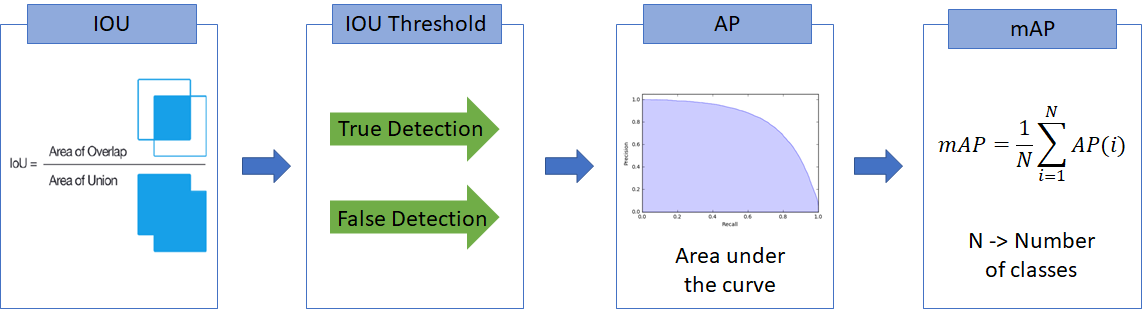
\includegraphics[width=0.9\textwidth]{Figures/mAP.png}
  \caption{Steps for obtaining the mean average precision (adapted from~\cite{unlu:real_app}).}
  \label{fig:map}
\end{figure}

The PASCAL VOC datasets contain 20 object categories (e.g., person, bicycle, dog) spread over 11k images, from which over 27k object instances are labeled with bounding boxes~\cite{jiao:obj_survey}. This benchmark considers only one IoU threshold of 0.5 to obtain the mAP. On the other hand, the COCO dataset is composed by 300k images with an average of 7 object instances per image from a total of 80 categories~\cite{zhao:obj_survey}. This benchmark considers ten IoU thresholds (from 0.5 to 0.95 with an interval of 0.05) and the mAP is obtained by averaging the mAPs calculated for each IoU threshold. Considering several IoU thresholds tends to reward models that are better at precise localization and penalizes the algorithms with a high number of bounding boxes with wrong classifications.

\vspace{-0.4cm}
\section{Comparison between object detectors}
\label{section:obj_det_comp}
\vspace{-0.1cm}

Several studies have been conducted for comparing the performance of the state-of-art object detectors~\citep{{jiao:obj_survey, liu:obj_survey, zhao:obj_survey}}. Object detectors can be divided into two categories: two-stage detectors (region proposal based) and one-stage detector (regression/classification based).

Two-stage detectors follow the traditional object detection pipeline by firstly scanning the whole scenario and then focusing on regions of interest. Thus, the first stage consists in generating region proposals (i.e., candidate bounding boxes). In the second stage, features are extracted from each candidate box in order to perform the classification and bounding box regression tasks. The most popular two-stage detectors are R-CNN, Fast R-CNN, Faster R-CNN, Mask R-CNN and R-FCN~\citep{{jiao:obj_survey, zhao:obj_survey, feng:obj_survey}}.

One-stage detectors treat object detection as a regression/classification problem by adopting a unified framework to obtain the labels and locations directly. These detectors map straightly from image pixels to bounding box coordinates and class probabilities by proposing predicted boxes directly from input images without the region proposal step. The most common one-stage detectors are Yolo and its successors Yolov2 and Yolov3, SSD and its successor DSSD and RetinaNet~\citep{{jiao:obj_survey, zhao:obj_survey, feng:obj_survey}}. 

The selection between one-stage and two-stage detectors resides on a choice between speed and accuracy. Two-stage detectors present higher localization and object recognition accuracy while one-stage detectors achieve higher inference speed. Table~\ref{tab:obj_det_comp} summarizes the mAP metric for both PASCAL VOC 2007 and COCO datasets and the inference time of each of the above-mentioned object detectors. For the COCO dataset, besides the official mAP metric (i.e., obtained from ten IoU thresholds), the mAP with only one IoU of 0.5 is also shown. 

\begin{table}[!htb]
    \footnotesize
    \centering
    \caption{Comparison of the performance of several object detectors.}
    \label{tab:obj_det_comp}
    \begin{tabular}{|c|c|c|c c|c c|c|c|}
    \hline
    
    \multirow{2}{*}{Type} & \multirow{2}{*}{Detector} & PASCAL VOC07 & \multicolumn{2}{|c|}{COCO} & \multicolumn{2}{|c|}{Inference time} & \multirow{2}{*}{Backbone} & \multirow{2}{*}{Hardware} \\ \cline{3-7}
    & & $mAP$ & $mAP$ & $mAP_{50}$ & ms & fps & & \\ \hline
    {\multirow{5}{*}{\rotatebox[origin=c]{90}{Two-stage}}} & R-CNN~\cite{feng:obj_survey} & 66 & --- & --- & 10000 & 0.1 & AlexNet & \multirow{16}{*}{Titax X GPU} \\ \cline{2-8}
    & Fast R-CNN~\cite{{jiao:obj_survey, feng:obj_survey}} & 70 & 19.7 & 35.9 & 2000 & 0.5 & VGG16 & \\ \cline{2-8}
    & Faster R-CNN~\cite{{jiao:obj_survey, feng:obj_survey}} & 73.2 & 21.9 & 42.7 & 167 & 6 & VGG16 & \\ \cline{2-8}
    & R-FCN~\cite{{jiao:obj_survey, zhao:obj_survey}} & \cellcolor{gray!25}83.6 & 29.9 & 51.9 & 170 & 5.9 & ResNet-101 & \\ \cline{2-8}
    & Mask R-CNN~\cite{{jiao:obj_survey, feng:obj_survey}} & --- & \cellcolor{gray!25}39.8 & \cellcolor{gray!25}62.3 & 303 & 3.3 & ResNeXt-101 & \\ \cline{1-8}
    
    {\multirow{13}{*}{\rotatebox[origin=c]{90}{One-stage}}} & YOLO~\cite{feng:obj_survey}  & 63.4 & --- & --- & \cellcolor{gray!25}22 & \cellcolor{gray!25}45 & GoogLeNet & \\ \cline{2-8}
    & YOLOv2-544~\cite{{jiao:obj_survey, zhao:obj_survey}} & 73.4 & 21.6 & 44 & \cellcolor{gray!25}25 & \cellcolor{gray!25}40 & DarkNet-19 & \\ \cline{2-8}
    & SSD-300~\citep{{jiao:obj_survey, zhao:obj_survey}} & 74.3 & 23.2 & 41.2 & \cellcolor{gray!25}21.7 & \cellcolor{gray!25}46 & \multirow{2}{*}{VGG-16} & \\ \cline{2-7}
    & SSD-512~\citep{{jiao:obj_survey, zhao:obj_survey}} & 76.8 & 26.8 & 46.5 & 52.6 & 19 & & \\ \cline{2-8}
    & SSD-321~\citep{{jiao:obj_survey, Redmon2018YOLOv3AI}} & --- & 28 & 45.4 & 61 & 16.4 & \multirow{4}{*}{ResNet-101} & \\ \cline{2-7}
    & SSD-513~\citep{{jiao:obj_survey, feng:obj_survey, Redmon2018YOLOv3AI}} & 76.8 & 31.2 & 50.4 & 125 & 8 & & \\ \cline{2-7}
    & DSSD-321~\citep{{jiao:obj_survey, zhao:obj_survey, Redmon2018YOLOv3AI}} & 78.6 & 28 & 46.1 & 85 & 11.8 & & \\ \cline{2-7}
    & DSSD-513~\citep{{jiao:obj_survey, Redmon2018YOLOv3AI}} & --- & 33.2 & 53.3 & 156 & 6.4 & & \\ \cline{2-8}
    & YOLOv3-320~\cite{Redmon2018YOLOv3AI} & --- & 28.3 & 51.5 & \cellcolor{gray!25}22 & \cellcolor{gray!25}45.5 & \multirow{3}{*}{DarkNet-53} & \\ \cline{2-7}
    & YOLOv3-416~\cite{Redmon2018YOLOv3AI} & --- & 31 & 55.3 & \cellcolor{gray!25}29 & \cellcolor{gray!25}34.5 & & \\ \cline{2-7}
    & YOLOv3-608~\cite{Redmon2018YOLOv3AI} & --- & 33 & 57.9 & 51 & 19.6 & & \\ \cline{2-9}
    & RetinaNet-500~\citep{jiao:obj_survey, Redmon2018YOLOv3AI} & --- & 34.4 & 53.1 & 90 & 11.1 & \multirow{2}{*}{ResNet-101} & \multirow{2}{*}{M40 GPU} \\ \cline{2-7}
    & RetinaNet-800~\citep{jiao:obj_survey, Redmon2018YOLOv3AI} & --- & 37.8 & 57.5 & 198 & 5 & & \\ \hline
    
    \end{tabular}
\end{table}
\vspace{-0.2cm}

The best performance for both PASCAL VOC and COCO datasets are achieved by two-stage detectors, namely R-FCN and Mask R-CNN. Higher frame rates are achievable with one-stage detectors such as YOLO (and its successors) and one version of the SSD detector. There are several versions available for the same detectors which mainly differ in the size of the input feature maps of the first layer. However, the topology of the network is the same for any version. For instance, YOLOv3 has three versions with input feature maps of  320x320, 416x416 or 608x608. Bigger input feature maps tend to lead to higher accuracy but lower speed. In the case of the SSD detector, some versions use VGG-16 which results in accelerated performance and others use ResNet-101 for higher accuracy. 

Within these detectors, YOLOv3 is the one that presents the best trade-off between accuracy and execution time (for the 320 and 416 versions). Therefore, this is the object detector that will be implemented in the scope of this work. 

\section{YOLOv3 detector}
\label{section:yolo}

Fig.~\ref{fig:yolov3} exemplifies the process flow of the YOLOv3 detector for an input feature map of 416x416. The input image is resized at the beginning of the process as the detector allows different input resolutions. The YOLOv3 network block is responsible for extracting features using the Darknet-53 backbone and for returning candidate bounding boxes from those features for three different scales (52x52, 26x26 and 13x13). Candidate bounding boxes are then filtered based on their objectness score and the score of each class. Finally, non-maximum suppression is used to remove multiple detections of the same object.  

\begin{figure}[!htb]
  \centering
  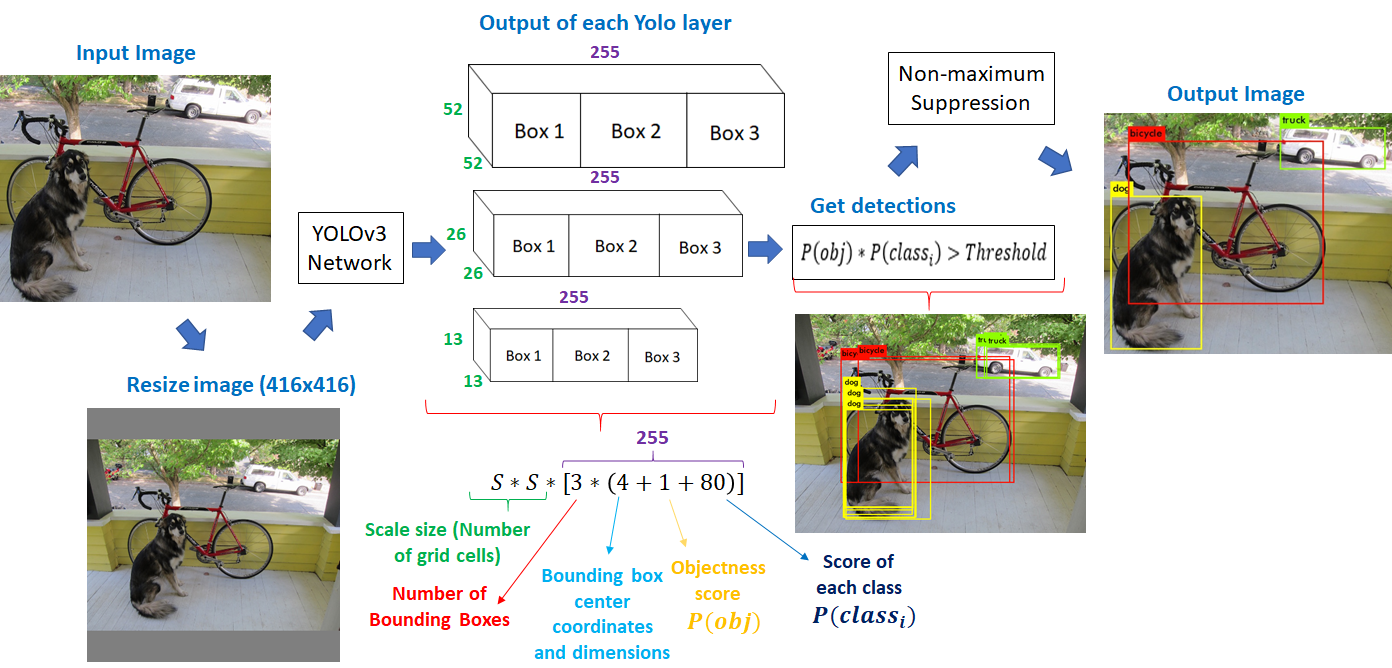
\includegraphics[width=\textwidth]{Figures/yolov3.png}
  \caption{YOLOv3 process flow.}
  \label{fig:yolov3}
\end{figure}

\subsection{YOLOv3 network}

The CNN-based YOLOv3 network is represented in Fig.~\ref{fig:yolov3_ntw}. This network is composed by 75 convolutional layers, 23 shortcut layers, 3 yolo layers, 2 upsample layers and 4 route layers, making a total of 107 layers. The two route layers after the yolo layers only copy the output of a former layer without concatenating with the output of the previous layer. All convolutional layers include batch-normalization and use Leaky ReLU (with $a$ = 0.1) as activation function, except from the convolutional layer exactly before of each yolo layer, which does not include batch-normalization and uses a linear activation function. There are no fully connected layers and convolutional layers with stride 2 are used instead of maxpool layers. One can also observe that every time the feature map is downsampled by a factor of four, the depth (i.e., number of channels) is duplicated. 3x3 convolutions are done with zero-padding in order to keep the same size between input and output feature maps.

\begin{figure}[!htb]
  \centering
  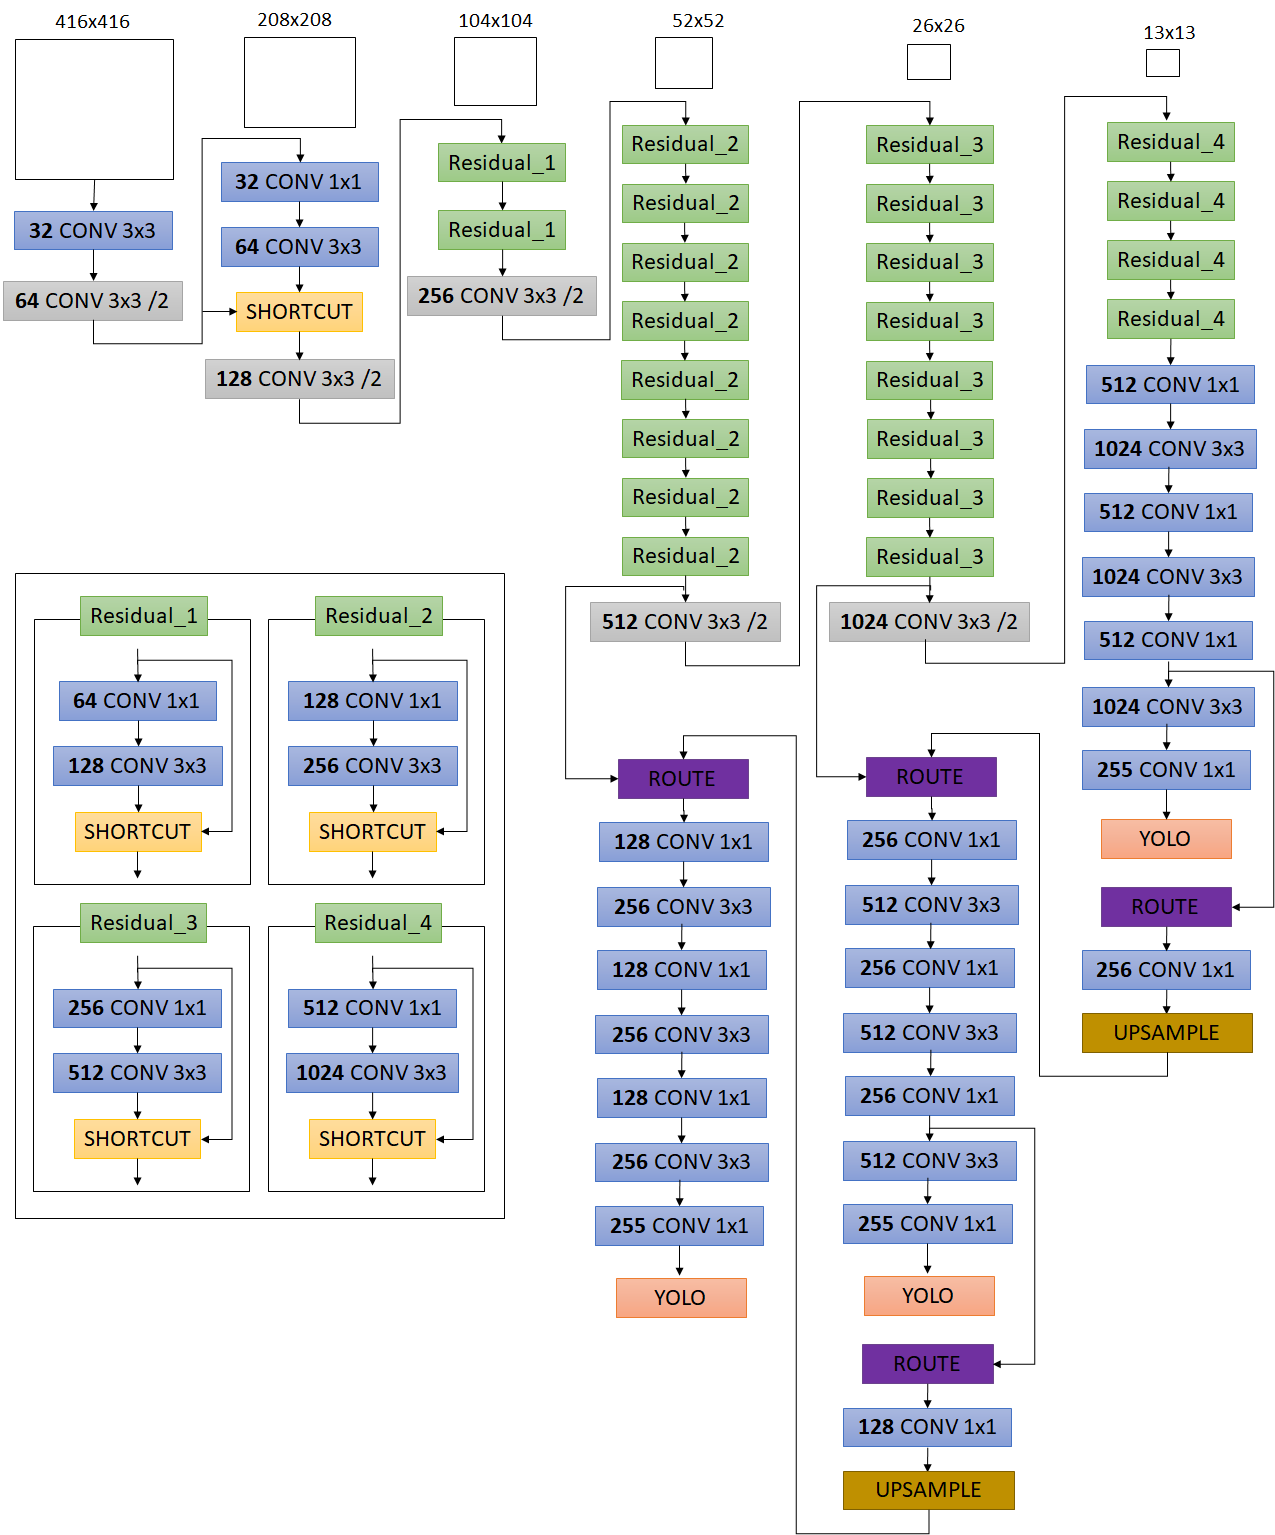
\includegraphics[width=0.9\textwidth]{Figures/yolov3_ntw.png}
  \caption{YOLOv3 Network.}
  \label{fig:yolov3_ntw}
\end{figure}

This network is inspired on some concepts from popular DNN models. For instance, the kernels are mostly 3x3 and 1x1 to reduce the number of weights as first introduced by GoogLeNet. A ResNet-alike structure is followed through the shortcut layers, thereby enhancing feature learning in deep networks. As the network goes deeper, due to downsampling the feature maps, small objects are difficult to detect.
Therefore, objects of different sizes are detected with different feature map scales through a structure similar to the Feature Pyramid Network (FPN)~\cite{zhao:obj_survey}. The FPN, represented in Fig.~\ref{fig:fpn}, is used for multi-scale feature learning and consists in merging, through the route layers, upsampled feature maps from deeper layers with feature maps of the same spatial size from early stages in order to capture both low and high-level information from objects~\cite{zhao:obj_survey}. YOLOv3 uses three scales: 52x52 to detect small objects, 26x26 to detect medium objects and 13x13 to detect big objects.

For each scale, the feature map is divided into a grid where each grid cell predicts 3 bounding boxes. The initial size of each bounding box (known as prior box) was set after using K-mean clustering in the training dataset~\cite{Redmon2018YOLOv3AI}. The sizes are then appropriately adjusted by the network. Each bounding box consists in the predictions of~\cite{Redmon2015YouOL}: 
i) the center of the box relative to the grid cell bounds (2 coordinates);  
ii) the width and height of the box relative to the whole image;
iii) the objectness (or confidence) score which indicates how likely the box contains an object and how accurate are its dimensions regarding to the ground truth box;
and iv) the conditional probability of every class given there is an object. As the YOLOv3 network is trained over the COCO dataset~\cite{Redmon2018YOLOv3AI}, the total number of classes is 80. Thus, each grid cell is composed by $3 * (2 + 2 + 1 + 80) = 255$ values, as specified in Fig.~\ref{fig:grid_cell}.

\begin{figure}[!htb]
  \centering
  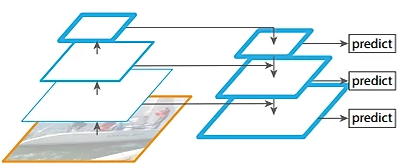
\includegraphics[width=0.5\textwidth]{Figures/fpn.png}
  \caption{Feature Pyramid Network structure~\cite{zhao:obj_survey}.}
  \label{fig:fpn}
\end{figure}

The logistic activation is used to constrain the center coordinates of the box to fall in the range of the grid cell (i.e., between 0 and 1). The objectness score is predicted using logistic regression (1 means perfect overlapping between predicted and ground truth boxes while 0 means no overlapping). For the class predictions, independent logic classifiers are also used. The application of the logistic activation in the predictions of each bounding box, excluding the width and height parameters, is performed by the \textbf{yolo layers}. This new layer added by the YOLOv3 network is used as the ending layer for each scale.

\begin{figure}[!htb]
  \centering
  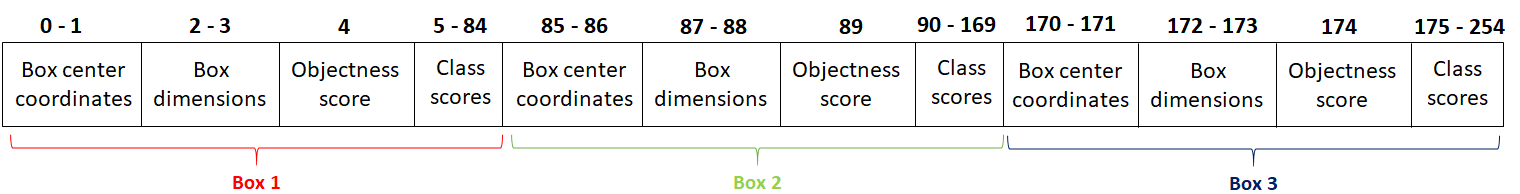
\includegraphics[width=\textwidth]{Figures/grid_cell.png}
  \caption{Constitution of each grid cell.}
  \label{fig:grid_cell}
\end{figure}
\vspace{-0.3cm}

\subsection{Detections phase}

After executing the YOLOv3 network block (Fig.~\ref{fig:yolov3}), there are several candidate bounding boxes for each scale, however, only a few of them correspond to true detections (depending on the number of objects in the image). The true detections correspond to the bounding boxes whose product between the objectness score and the conditional probability of each class is above a given threshold (the default value is 0.5). The bounding boxes can be multilabeled, i.e., can have more than one class. 

Due to detecting objects with three different scales and with three bounding boxes per grid cell, multiple bounding boxes of the same object might be found. The non-maximum suppression is used to remove these multiple detections and consists in the following algorithm~\cite{Redmon2015YouOL}:
\vspace{0.3cm}

\begin{algorithm}[H]
\setstretch{1}
 1) Select bounding box with the highest confidence score \\
 2) Calculate the IoU between selected box and all the remaining boxes \\
 3) Discard boxes whose IoU is greater than a certain threshold (default value is 0.45)\\
 4) Repeat steps 2-4 for the next highest score box until processing all remaining boxes
 \caption{Non-maximum suppresion}
\end{algorithm}

 
\subsection{YOLOv3-Tiny network}

The YOLOv3 network comprises a total of nearly 62 million parameters. The author of this detector~\cite{Redmon2018YOLOv3AI} proposed an alternative network for constrained environments called YOLOv3-Tiny which in turn has a total of approximately 8.8 million parameters. This smaller model presents a mAP (for one IoU of 0.5) of 33.1\% in the COCO dataset and runs at a frame rate of 220 fps in the Titan X GPU. Thus, this version is faster but also less accurate than any other detector in Table~\ref{tab:obj_det_comp}. In the scope of this work, this network can be used as a starting point for acceleration before moving to the YOLOv3 network. 

As represented in Fig.~\ref{fig:yolov3_tiny_ntw}, the YOLOv3-Tiny is composed by 13 convolutional layers, 6 maxpool layers, 2 route layers, 2 yolo layers and 1 upsample layer. In comparison with YOLOv3, this network uses maxpooling instead of convolutions with stride 2 to downsample the feature maps. Besides that, objects are detected with only 2 scales (26x26 and 13x13). No shortcut layers are used.  

\begin{figure}[!htb]
  \centering
  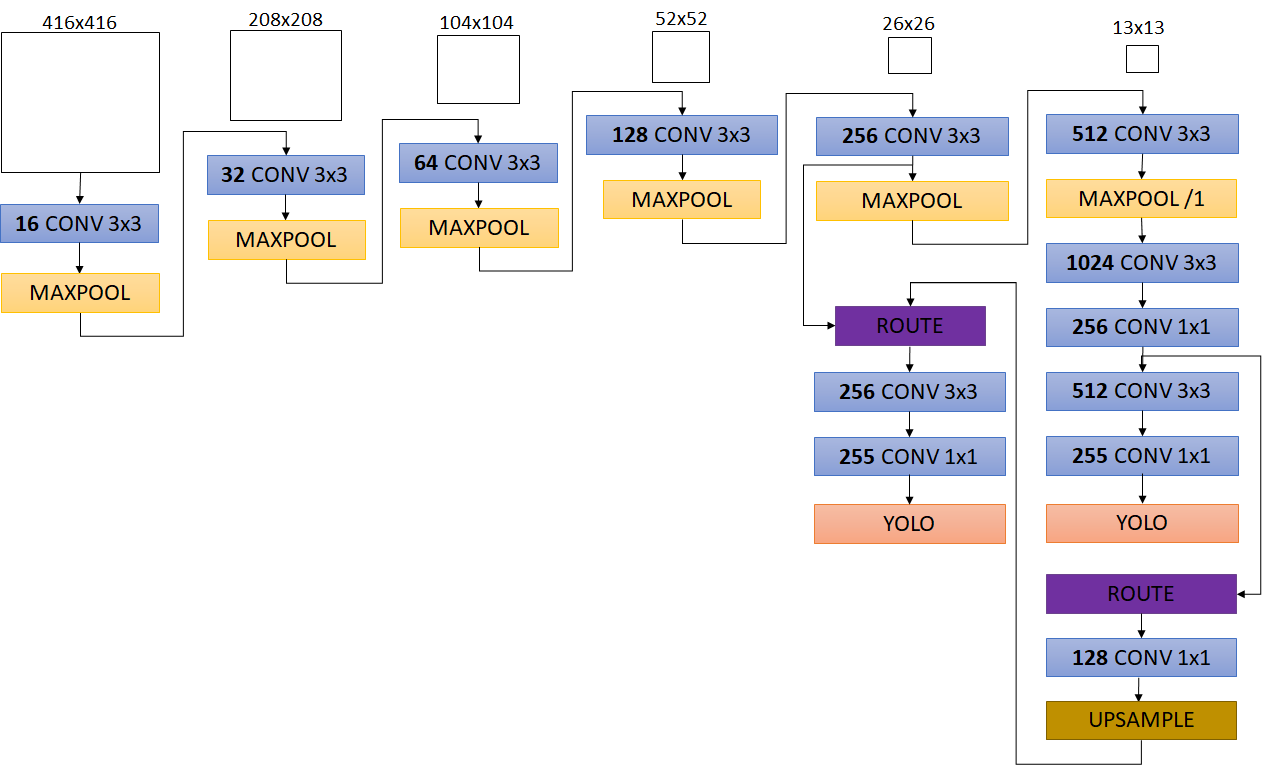
\includegraphics[width=0.85\textwidth]{Figures/tiny.png}
  \caption{YOLOv3-Tiny Network.}
  \label{fig:yolov3_tiny_ntw}
\end{figure}

\subsubsection{Final remarks}

The backbone for feature extraction of the state-of-art object detectors are based on the popular CNNs introduced in the previous chapter. PASCAL VOC and COCO are the most common benchmarks for the evaluation of object detectors where YOLOv3 presents the best trade-off between accuracy and execution time. For this work, the lighter YOLOv3-Tiny network will be initially accelerated using the architecture introduced in the next chapter.   

\chapter{CGRA-based accelerator}
\label{chapter:cgra}

In this chapter, the fundamentals about Coarse Grained Reconfigurable Arrays
(CGRAs) and why they can be used for accelerating CNNs are briefly
explained. The Deep Versat CGRA architecture, which will be used in this work
for accelerating the YOLOv3 detector, is described. The chapter ends with a
basic example of the implementation of a 2D convolution using a single layer of
the Deep Versat core.

\section{CGRA architecture}
\label{section:cgra_arch}

A CGRA is a collection of programmable functional units (FUs) and embedded memories interconnected by programmable switches~\cite{lopes:versat}. The interconnections are reconfigurable at run-time, which allows to form different hardware datapaths to accelerate distinct computations for the same application. CGRAs are reconfigurable at the word-level and the hardware units can be programmed in any execution cycle.

Typically, CGRAs consist of a reconfigurable array, which is mainly used to accelerate program loops, and a conventional CPU, which executes the non-loop code of a given application and controls the configuration of the array. Thus, CGRAs can be used as hardware co-processors to accelerate parts of the algorithms that are slow or energy inefficient in regular CPUs~\cite{valter:deep_versat}.  

The FPGA-based architecture for accelerating CNNs proposed on previous works, which was studied in section \ref{subsection:acc_opt}, is the same as the CGRA architecture. Both consist of a spatial array of processing elements (i.e., functional units) with data flowing through an interconnection network and memory is located as close as possible to the computational units~\cite{auto_tuning_cgra}. 

The reconfigurable array is suitable for accelerating program loops, which fits with the implementation of the convolutional layers. For all these reasons, a CGRA-based architecture can be used for accelerating CNNs. For instance,~\cite{alexnet_cgra} implemented the AlexNet network in a CGRA by using 16 PEs and 9 parallel multipliers with fixed-point arithmetic of 8 bits for the image pixels, 16 bits for the weights, bias and output feature maps and 32 bits for intermediate results, achieving a throughput of 141 GOPs, which is comparable with the ones obtained in Table~\ref{tab:comp_fpga_acc}. An auto-tuning compiler to map CNNs in CGRA architectures by exploring loop optimization techniques is proposed in~\cite{auto_tuning_cgra} . The author claims that the developed CGRA outperforms, in terms of energy per inference, other ARM-based accelerators.

\section{Deep Versat}
\label{section:versat}

Versat \cite{lopes:versat} is a 32-bit CGRA architecture developed at the INESC-ID Research Institute capable of being configured on the fly, without using pre-compiled configurations, through partial reconfiguration. The ability of generating configuration sequences from stored routines, instead of storing the configuration itself, allows to exploit the similarity between configurations as only distinct bits need to be changed, which results in a faster and less energy consuming configuration. 

Versat is composed of FUs organized in a full mesh topology, which limits the number of FUs that an application could use, due to the increase of the circuit delay caused by the selection multiplexers. To overcome this limitation, a multi-layer architecture composed of a set of Versats, called Deep Versat, was proposed in a master thesis~\cite{valter:deep_versat}. With more layers, programs can use more FUs. Layers are stacked in a ring structure, as shown in Fig.~\ref{fig:deep_versat}, to limit the number of connections and prevent a frequency drop.

\vspace{-0.3cm}
\begin{figure}[!htb]
  \centering
  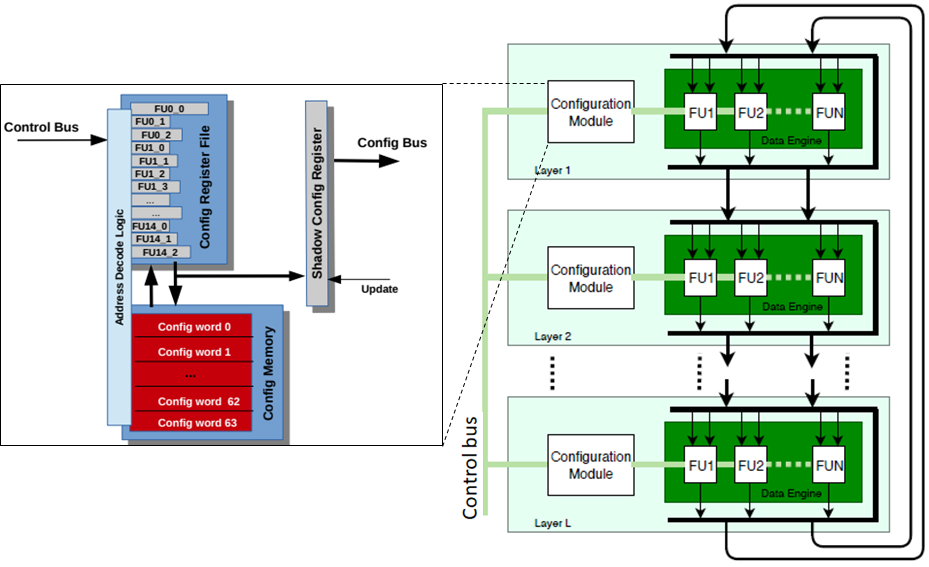
\includegraphics[width=0.85\textwidth]{Figures/deep_versat.png}
  \caption{Deep Versat architecture (adapted from~\cite{valter:deep_versat}).}
  \label{fig:deep_versat}
\end{figure}
\vspace{-0.15cm}

%FIX é Control Bus (do picorv) na figura e não Config Bus. Nota que não serve apenas para
%config mas tb para dar o start e ver se acabou. Do lado esquerdo da figura está
%certo e diz Control bus. Config. bus é o que liga o CM ao DE --> (DONE)

Each Versat has a data engine and a configuration module. In the data engine,
the FUs are interconnected by a data bus which concatenates the 32-bit output of
each FU of the current and of the previous layer (memories have two 32-bit
outputs as they are dual-port). As the interconnection follows a full mesh
topology, each FU can select any section from the data bus by means of a
programmable multiplexer, depending on the configuration defined in the
configuration bus.

The configuration module is composed by (1) the Configuration Shadow Register,
which stores the configuration currently being executed by the respective data
engine, (2) the Configuration Register File, which holds the next configuration,
and (3) the Configuration Memory, which saves frequently used configurations. The configuration bus connects the data engine and the configuration
module.

Currently, the functional units available include dual-port memories, arithmetic
logic units (ALUs), multipliers, multiplier and accumulators (called MulAdd) and
barrel shifters. The number of FUs is configured at compile time. Each FU holds
different configuration parameters based on their functionality: \\

\vspace{-0.4cm} \textbf{Dual-port memory}: Besides the 2 input and output ports,
each Versat memory has two Address Generation Units (AGUs) which consist in two
cascaded counters that allow for the execution of two nested loops in one
configuration. The AGU can be programmed to generate the address sequence for
accessing data from the memory during the execution of a program loop or to
generate a counter to control, for example, a MulAdd. The parameters are
described in Table~\ref{tab:versat_agu_param}.

%FIX below note that the base addresses are not parameters of the FU but of the
%system. The FU itself does not store its base address. Only the system needs to
%know it to be able to access it. However in the software API it makes sense to
%associate each FU base address with the FU class. --> (DONE)

\begin{table}[!htb]
    \footnotesize
    \centering
    \caption{Parameters of the dual-port memories.}
    \label{tab:versat_agu_param}
    \begin{tabular}{|c|c|c|c|}
    \hline
    Parameter   &  Description                          & Parameter     &  Description                                      \\ \hline
    start       & Memory start address                  & per           & N.º of inner loop iterations (period)             \\ \hline
    iter        & N.º of outer loop iterations          & duty          & N.º of cycles in a period where memory is enabled \\ \hline
    incr        & Increment of the inner loop           & sel           & Address of the input FU                           \\ \hline
    delay       & N.º of clock cycles before AGU starts & shift         & Additional increment at the end of each period    \\ \hline
    ext         & Flag for bypassing the AGU            & \multicolumn{2}{c|}{}                                                   \\ \hline
    \end{tabular}
\end{table}

%The nested loops computation and respective parameters of the AGU are represented in Fig. \ref{fig:agu_nested_loops}. 

%\begin{figure}[!htb]
%  \centering
%  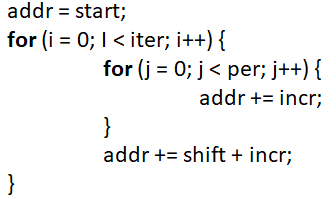
\includegraphics[width=0.3\textwidth]{Figures/versat_agu.png}
%  \caption{AGU nested loops computation.}
%  \label{fig:agu_nested_loops}
%\end{figure} 

\textbf{ALU / Multiplier}: These FUs have 3 parameters: the two input operand addresses and the type of operation. In the case of the ALU,
the most common operations include logic operations (e.g. AND, OR) and
additions. The multiplier has a latency of three clock cycles and allows to
choose the upper or lower 32-bit part of the 64-bit multiplication result.\\

\vspace{-0.4cm} \textbf{Barrel shifter}: The barrel shifter has a latency of 1 clock cycle and has 3 parameters: the address of the operand to be shifted, the size of the shift and the type/direction of the shift (e.g, right/left, logic/arithmetic).\\

\vspace{-0.4cm} \textbf{MulAdd}: The MulAdd was also added by~\cite{valter:deep_versat}. This FU has 4 configuration parameters: the two operand addresses, the reset and the type of operation. The reset controls how many accumulations to perform and can be applied with a counter from a memory AGU.  

%FIX the counter is not a parameter in the hw (is it in the sw?). The FU has an
%input to control when it resets. -> DONE

\subsection{System integration}

As previously mentioned, a CGRA is typically accompanied by a CPU. As shown in Fig.~\ref{fig:deep_versat_system}, Deep Versat is controlled by a RISC-V soft-processor. In this system, the processor accesses peripherals through its memory bus. Deep Versat can be seen as two peripherals, one for the control bus to start its execution and manipulate the configuration registers and another one for the data bus, which is used for data transfers. The UART module is another peripheral mainly used for debugging.

\begin{figure}[!htb]
  \centering
  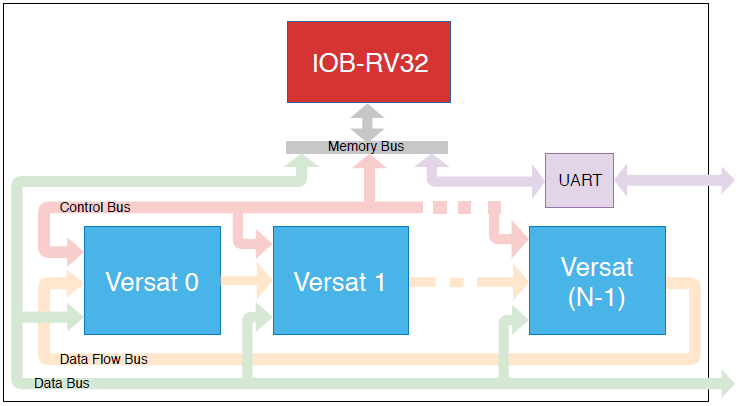
\includegraphics[width=0.6\textwidth]{Figures/deep_versat_system.png}
  \caption{Deep Versat system~(\cite{valter:deep_versat}).}
  \label{fig:deep_versat_system}
\end{figure}

%\vspace{-0.5cm}
\subsection{Basic implementation}

The RISC-V processor is programmed with a standard GNU toolchain, which contains compilers for C and C++. Therefore, Deep Versat also includes an API in C++ to enhance its configuration process. To show the usage of this API, a simple 2D convolution, using a single Versat layer, between a 5x5 feature map and a 3x3 kernel (without zero-padding) is exemplified in Fig.~\ref{fig:convolution_versat}. 

The feature map and the kernel are stored in different memories (mem0 and mem1). To read a 3x3 block from the feature map, a correct manipulation of the parameters in Table~\ref{tab:versat_agu_param} is needed. The parameters $iter$, $per$ and $duty$ are set to 3 in order to read one pixel per clock cycle across the 3 columns and 3 lines. The shift must be 2 to read the next row as data is stored in row-major order. For the kernel, 9 consecutive positions from mem1 are read. The second port (B) of this memory is used to generate a counter from 0 to 8 to control the number of accumulations in the MulAdd, whose inputs are connected to both memories. The results are stored in another memory (mem2). Finally, the loops for iterating through the feature map are defined in software to configure the start address of the read memories and to run the Versat at each iteration. 

\vspace{+0.1cm}

\begin{figure}[!htb]
  \centering
  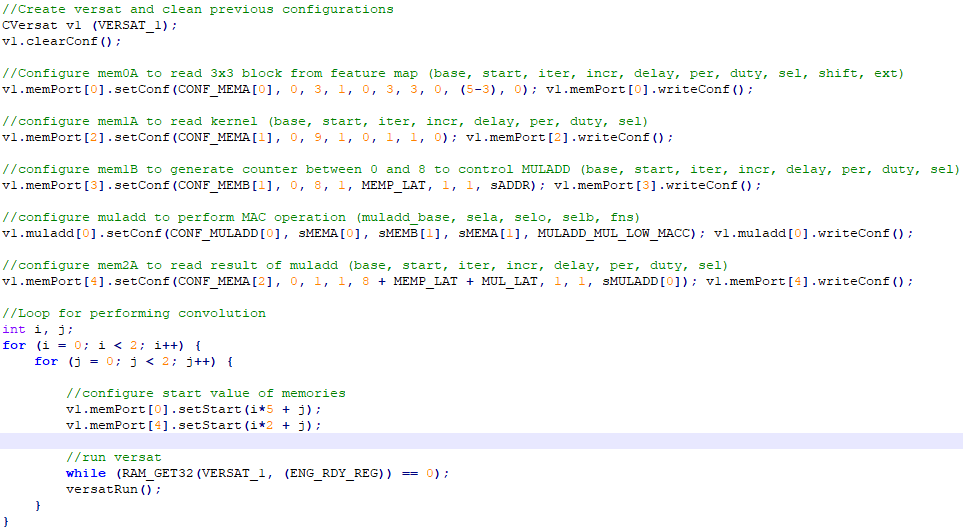
\includegraphics[width=\textwidth]{Figures/versat_convolution.png}
  \caption{Example of 2D convolution with one Versat.}
  \label{fig:convolution_versat}
\end{figure}
\vspace{-0.4cm}

\subsubsection{Final remarks}

This simple example showed how to accelerate loops using a single Versat layer. By using more layers from the Deep Versat architecture and by applying loop optimization techniques, convolutional layers from complex CNNs such as the YOLOv3 detector can be accelerated. In the next chapter, the proposed methodology and the expected planning of this work are described.

\chapter{Proposed methodology and planning}
\label{chapter:methodology}

The main goal of this work is to implement and demonstrate a real-time object detector in a FPGA-based development board. Taking into account the study performed in chapter \ref{chapter:object_detection}, the YOLOv3 detector presents the best trade-off between accuracy and execution time. The Deep Versat system, introduced in chapter \ref{chapter:cgra}, alongside the techniques for CNN acceleration in FPGAs studied in chapter \ref{chapter:DNN}, will be used to implement the detector.

\section{Infrastructure}
\label{section:infrastructure}

The development board available for this work is the Kintex UltraScale KU040~\cite{fpga}. To receive images in real-time, the cost-effective OV7670 camera module~\cite{camera} was chosen as it can be easily connected to the PMOD modules of the board. This camera operates at maximum 30 fps and has a maximum resolution of 640x480 pixels. Given the interfaces available on the board, the HDMI interface was selected to display the resulting images in a monitor. The proposed infrastructure is represented in Fig.~\ref{fig:infrastructure}. 

\begin{figure}[!htb]
  \centering
  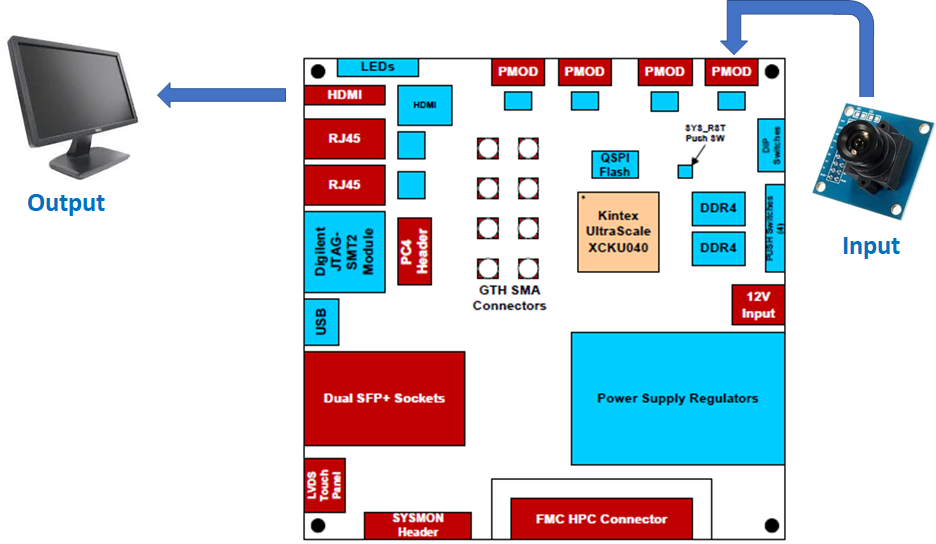
\includegraphics[width=0.85\textwidth]{Figures/fpga_system.png}
  \caption{Composition of the proposed infrastructure (adapted from~\cite{fpga}).}
  \label{fig:infrastructure}
\end{figure}

\subsection{OV7670 camera module}

The pinout of the camera is represented in Table~\ref{tab:ov7670}. The camera has two different communication protocols: one for its configuration and another for data acquisition. The pins SDIOD and SDIOC are used for configuring the camera using a specific protocol similar to I2C. Possible configurations include the data output format (e.g., RGB565, YCbCr 4:2:2), the frame resolution (e.g., 640x480, 320x240) and the frame rate. For this work, the camera will be configured in the RGB565 format with a resolution of 640x480 and a frame rate of 30 fps.

\begin{table}[!htb]
    \footnotesize
    \centering
    \caption{Parameters of the dual-port memories.}
    \label{tab:ov7670}
    \begin{tabular}{|c|c|c|c|c|}
    \hline
    Type & Pin & Description & Pin &  Description \\ \hline
    Supply & VDD & Power supply & GND & Ground \\ \hline
    Input/Output & SDIOD & Control bus data & \multicolumn{2}{c|}{} \\ \hline
    \multirow{2}{*}{Input} & SDIOC & Control bus clock & XCLK & System clock \\ \cline{2-5}
    & RESET & Reset (active low) & PWDN & Power down (active high) \\ \hline
    \multirow{2}{*}{Output} & VSYNC & Vertical synchronization & HREF & Horizontal synchronization \\ \cline{2-5}
    & PCLK & Pixel clock & D0-D7 & Pixel parallel output \\ \hline
    \end{tabular}
\end{table}

Changing the configuration corresponds to updating the value of a specific register in the camera module. When idle, both SDIOC and SDIOD are at logical one. The data transmission starts by driving the SDIOC pin at logical zero. A logical one during data transmission indicates that one bit was sent. The SDIOD pin can only change while SDIOC is at logical zero. After transmitting the address of the register and the value to be updated, the pins are driven at logical one, indicating the end of the transmission.

The pixel data is transmitted in parallel (8 bits). First, a frequency between 10 and 48 MHz must be supplied to the XCLK pin~\cite{camera}. As shown in Fig.~\ref{fig:data_acquisition}, the 640 pixels that form one row must be captured while HREF is at logical one and the 480 rows are acquired while VSYNC is at logical zero. The data must be sampled at the rising edge of the PCLK signal. For the RGB565 format, two clock cycles are needed to collect each pixel. The reset and power down signals are kept at logical zero and logical one.

\begin{figure}[!htb]
  \centering
  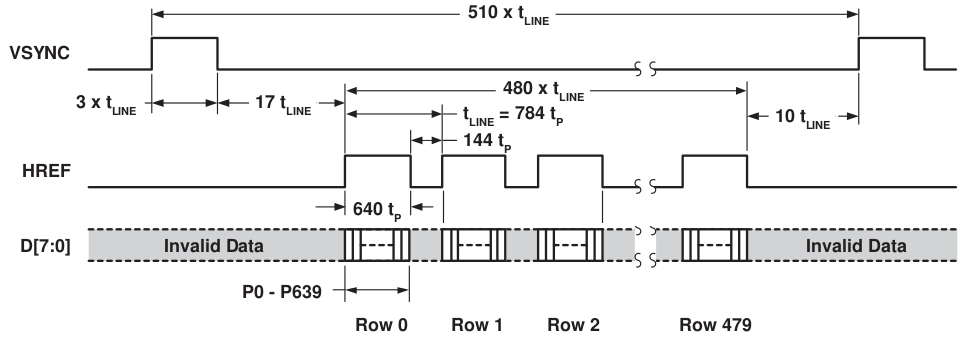
\includegraphics[width=0.85\textwidth]{Figures/camera_data_acquisition.png}
  \caption{Protocol for the camera data acquisition~\cite{camera}.}
  \label{fig:data_acquisition}
\end{figure}

\vspace{-0.2cm}
\subsection{HDMI module}

The board has an ADV7511 HDMI transmitter~\cite{hdmi} to drive the interface. Although the ADV7511 module accepts 36 bits per pixel, the board is only connected to 16 pixels (from bit 8 to bit 23)~\cite{fpga}. As a consequence, the format of the data must be YCbCr 4:2:2. This implies a color space conversion from the RGB format of the camera to the YCbCr format of the HDMI interface~\cite{color_conversion}:

\begin{equation}
    %\syslineskipcoeff{1}
    \normalsize 
    \systeme*{ Y = 16 + \frac{65.738}{256} \times R + \frac{129.057}{256} \times G + \frac{25.064}{256} \times B, Cb = 128 - \frac{37.945}{256} \times R - \frac{74.494}{256} \times G + \frac{112.439}{256} \times B, Cr = 128 + \frac{112.439}{256} \times R - \frac{94.194}{256} \times G - \frac{18.285}{256} \times B}
\end{equation}
\vspace{+0.2cm}

The video streams have active video periods and blanking periods, as represented in Fig.~\ref{fig:active_video} . Only the active video is shown on the display. When transmitting video, the signals HSYNC (horizontal synchronization), VSYNC (vertical synchronization) and DE (data enable) must be generated.

\begin{figure}[!htb]
  \centering
  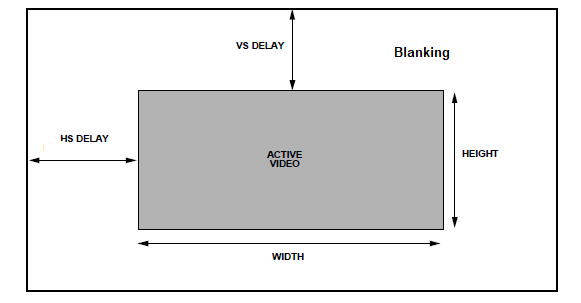
\includegraphics[width=0.7\textwidth]{Figures/active_video.png}
  \caption{Active video (adapted from~\cite{camera}.)}
  \label{fig:active_video}
\end{figure}

A logic one DE indicates an active pixel (i.e., the visual part of the video signal) and a logic zero DE indicates the blanking period of the video signal. The generation of the DE is represented in Fig.~\ref{fig:hdmi_signals}. The range of values for the synchronization signals depends on the resolution being used. For configurations such as the data format, the I2C protocol is used.

\begin{figure}[!htb]
  \centering
  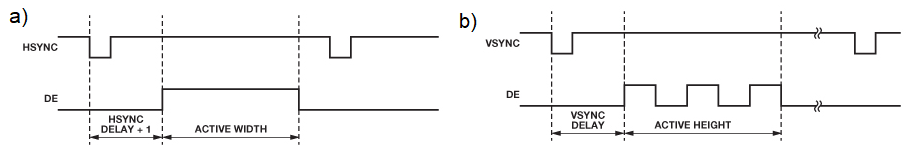
\includegraphics[width=\textwidth]{Figures/hdmi_signals.png}
  \caption{a) Horizontal and b) vertical DE generation (adapted from~\cite{camera}).}
  \label{fig:hdmi_signals}
\end{figure}

The camera and HDMI modules will be developed in Verilog. These modules will be integrated as peripherals in the Deep Versat system as represented in Fig.~\ref{fig:final_system}. 

\begin{figure}[!htb]
  \centering
  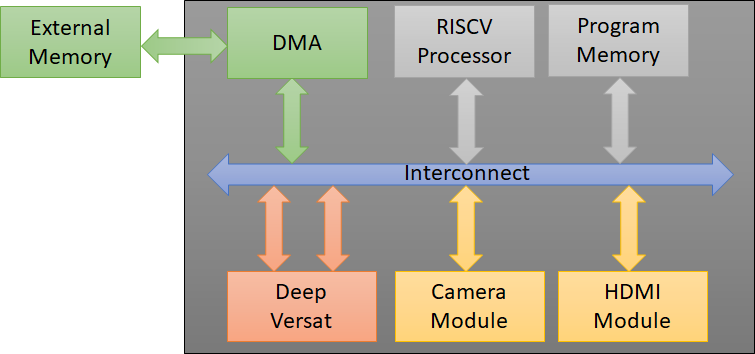
\includegraphics[width=0.6\textwidth]{Figures/final_system.png}
  \caption{Integration of the modules in the Deep Versat system.}
  \label{fig:final_system}
\end{figure}

\section{Planning}
\label{section:planning}

This thesis work is planned for a period of nine months, as shown in the Gantt Chart presented in Fig. \ref{fig:planning}. The first task will consist in implementing a software-only version of the YOLOv3 detector in the RISC-V processor to be used as baseline. As this processor currently does not support floating point operations, the application will need to be already converted to fixed point arithmetic by applying a pre-defined quantization. The detector will initially be based on the YOLOv3-Tiny network.

For the second task, the convolutional layers will be accelerated using the Deep Versat architecture. Following the approach in previous works, a design space exploration will be conducted in order to find the best parameters for the loop optimization techniques, namely the unroll and tiling factors.

Furthermore, a study will be conducted in order to measure the impact of implementing the other layers and other routines of the detector (e.g., image resize, non-maximum suppression) in the RISC-V processor. If after accelerating the convolutional layers, the bottleneck of the application resides on any of these routines, then hardware-based alternatives will have to be considered. For instance, the logistic operation performed by the yolo layers can be approximated by using pre-defined values stored in LUTs. 

The following two tasks will focus on the deployment of the camera and HDMI modules for the infrastructure proposed in this chapter. Finally, the system will be fully integrated and tested. The thesis will be written throughout the implementation of the work. 

\begin{figure}[!htb]
  \centering
  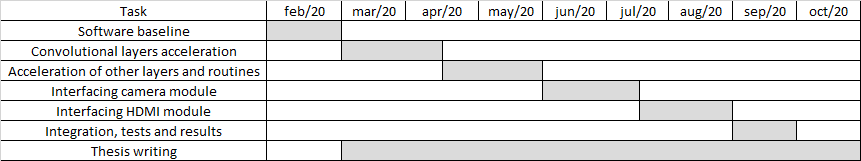
\includegraphics[width=\textwidth]{Figures/gantt.png}
  \caption{Planning of the thesis.}
  \label{fig:planning}
\end{figure}

\subsubsection{Final remarks}

The expected results with the development of this work include the infrastructure for receiving images from the OV7670 camera in real-time and displaying the resulting images from the YOLOv3 detector in an HDMI monitor. For the YOLOv3-Tiny network, the expected frame rate should be near the maximum frame rate of the camera (i.e., 30 fps).  

%\cleardoublepage

%%%%%%%%%%%%%%%%%%%%%%%%%%%%%%%%%%%%%%%%%%%%%%%%%%%%%%%%%%%%%%%%%%%%%%%%%
%                                                                      %
%     File: Thesis_Implementation.tex                                  %
%     Tex Master: Thesis.tex                                           %
%                                                                      %
%     Author: Andre C. Marta                                           %
%     Last modified :  2 Jul 2015                                      %
%                                                                      %
%%%%%%%%%%%%%%%%%%%%%%%%%%%%%%%%%%%%%%%%%%%%%%%%%%%%%%%%%%%%%%%%%%%%%%%%

\chapter{Proposed Work}
\label{chapter:implementation}

The proposed project consists in the development of a Yolov3 CNN application for
Deep Versat, with focus on the convolutional layer, that represents the majority
of computations in CNNs.

This involves the design of a set of acceleration datapaths for Deep Versat,
which, in turn, may require the improvement of the existing FU set. The overall
goal is to accelerate the execution of the application up to 30 images per
second in order to achieve video speed.

% intro to several sections

\section{Yolov3 Software Modeling}
\label{sec:yolov3_baseline}
The Yolo networks use Darknet~\cite{darknet13}, an open source neural network in
C and CUDA, which does not have support for reduced precision
operands. Therefore, the development of a code base that facilitates the
evaluation of the Yolov3 network in terms of operand precision becomes a
requirement.

This evaluation is necessary to verify the accuracy of the network with reduced
precision operands and to measure the ranges of the activations at each
layer. Only with this analysis it is possible to implement an effective
quantization based on DFP (section~\ref{sec:quantization}), which is necessary
for deep networks.


\section{Baseline Hardware System}
\label{sec:hw_baseline}
In order to establish a baseline for the performance of the Deep Versat, the
system presented in Fig.~\ref{fig:baseline_hw_system} will be used. The
architecture uses as base the system in~\cite{VMario:Deep_Versat}.

The main difference from the system in~\cite{VMario:Deep_Versat} is the addition
of the DMA connection between the Deep Versat and the external memory. As
discussed in~\ref{sec:Versat_controller}, this change frees the host system
during data transfers.

A RISC-V processor is used as the host and controller for Deep Versat. This soft
processor treats each other block in the system as a memory mapped
peripheral. The processor is also tasked to execute the parts of the application
that are not accelerated by the Deep Versat.

The UART block is useful in development for debugging purposes, as it is a
practical way to receive feedback from the system into a console on an external
computer.

Deep Versat has been programmed with a convolutional layer for accelerating a
hand written digit recognition application~\cite{VMario:Deep_Versat}. This
implementation uses Versat's current set of FUs, which are reconfigured many
times to form datapath configurations as discussed in~\ref{sec:Deep_Versat}.

With this implementation it is possible to both verify the correct functioning of
the system and all its components, as well as establishing a baseline in terms
of performance for convolution acceleration.

\begin{figure}[!htb]
	\centering
	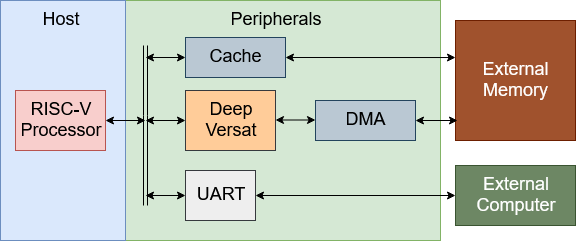
\includegraphics[width=0.6\textwidth]{Figures/baseline_HW_system.png}
	\caption[Caption for figure in TOC.]{Baseline hardware system}
	\label{fig:baseline_hw_system}
\end{figure}
%FIX o que liga o risc-v a memoria externa é uma cache e não um dma. Não existe Program Memory, é a cache. (FIXED)

\section{Datapath Proposal for Convolutional Layers}
\label{sec:planned_datapath_for_conv_layers}
The acceleration of convolutional layers will start with the proposal of a
datapath architecture, based on the analysis
in~\ref{sec:Datapath_Optimizations}. The accelerator presented
in~\ref{sec:proposed_accelerator} is a promising starting point for the
architecture.

The designed datapaths may require the development of new of FUs or tweaking of
the existing ones. There is then the challenge of mapping the convolution
datapaths into the Deep Versat architecture using the modified FU set.  After
that, the convolution layer can be tested and compared with the baseline
results. The work reported in this section is the main focus of the project and
is expected to be the most time consuming task.

\section{Experimental Validation with Yolo Networks}
\label{sec:experimental_yolo_validation}
With a new Convolutional Layer tested and working properly, the next test is to
execute the Tiny-Yolov3 network (section~\ref{sec:tiny-yolov3}) on the
system. This represents an intermediate step due to the reduced requirements of
this network, when compared with the full Yolov3. As a general goal for the
project, processing 30 images per second would be ideal, although this objective
may not be achieved.


%FIX: Não percebi porque é preciso desenvolver uma FU para conv. Já existe o MAC tal
%como explicaod no Alg1. O que podemos ter de mexer é nas AGUs para aumentar o
%numero de loops executados no Deep Versat


\section{Work Calendarization}
\label{sec:tasks_GANT}
In Fig.~\ref{fig:tasks_callendar} it is presented a GANT chart outlining the
calendarization of the planned work.


%FIX: altera o planeamento de acordo uma vez que não vejo a tarefa de desenhar uma FU como dominante.

\begin{figure}[!htb]
	\centering
	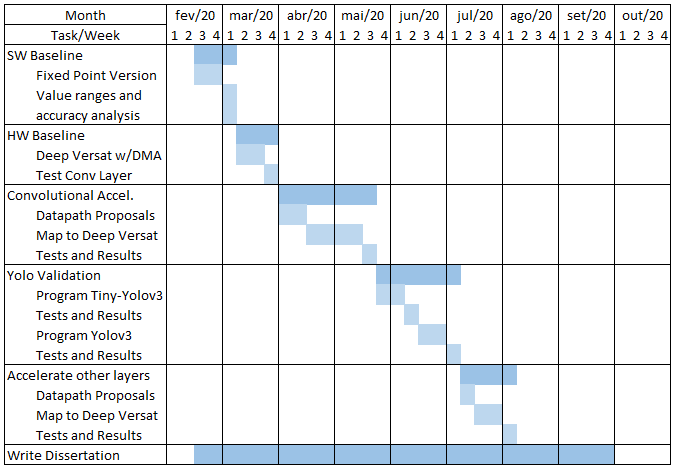
\includegraphics[width=0.95\textwidth]{Figures/dummy_GANT.png}
	\caption[Caption for figure in TOC.]{Work Planning}
	\label{fig:tasks_callendar}
\end{figure}


%\begin{itemize}
%	\item Proposed Methodologies
%	\subitem Outline of base system
%	\subitem PE in Versat architecture
%	\subitem General PE architecture proposal
%	\item Expected Results
%	\subitem Target performances and goals (accuracy, fps, networks)
%	\item Work planning table (GANT)
%\end{itemize}


 % file "Thesis_Implementation.tex"
%\cleardoublepage

%\input{Thesis_new_file} % add new .tex files for new chapters
% \cleardoublepage

%\input{Thesis_new_file} % add new .tex files for new chapters
% \cleardoublepage

%\input{Thesis_new_file} % add new .tex files for new chapters
% \cleardoublepage

%%%%%%%%%%%%%%%%%%%%%%%%%%%%%%%%%%%%%%%%%%%%%%%%%%%%%%%%%%%%%%%%%%%%%%%%%
%                                                                      %
%     File: Thesis_Results.tex                                         %
%     Tex Master: Thesis.tex                                           %
%                                                                      %
%     Author: Gonçalo Santos                                           %
%     Last modified : 20 Oct 2018                                      %
%                                                                      %
%%%%%%%%%%%%%%%%%%%%%%%%%%%%%%%%%%%%%%%%%%%%%%%%%%%%%%%%%%%%%%%%%%%%%%%%

\chapter{Results}
\label{chapter:results}

The aim of this work is to produce a workable {\bf C} language
compiler for the {\it Versat} architecture using the {\it picoVersat}
instruction set.
The success can be measured by the number of {\bf C} language
constructs that are working properly.
Consequently, testing is of primordial importance, as are the range
of tests used to exercise the compiler.

\section{Functionality}

The compiler, as far the tests were comprehensive,
supports all {\bf C} language integer constructs.
Limitations are listed below.

Since the processor instruction set is reduced, as are the
number of {\bf lcc} terminals to be implemented by the compiler,
the testing of each operation, on its own, is strait
forward.
Testing sequences of such operations may prove more
difficult to test, since different {\bf C} programs
can produce different selection matches.

\section{Testing}

In the test of a compiler, where a small change can affect the
generation of multiple instructions, a good set of
regressive tests is very important.
In order to automate the process, a {\tt test/} directory
was setup.
This directory includes a set of {\bf .c} test files and
the expected output {\bf .out}.

The {\tt Makefile} compiles, executes and compares the new
result with the previously stored result.
All differences in output are printed and can then be analyzed.

Since the output from {\bf iverilog} includes the number
of clocks spent, it is easy to compare whether the changes in the
compiler result in improvements, or in performance degradation.

Some tests are very simple and its output can be easily predicted.
To make testing even simpler, the return value of the {\tt main}
routine is printed, unless the {\sc NORET} environment variables
is defined. Upon return from the {\tt main} routine, the lowest
nibble is printed as an {\sc ASCII} starting at $0$.
This means that values between $10$ and $15$ are printed as
the {\sc ASCII} character at the respective offset, namely the
sequence: \verb|:|, \verb|;|, \verb|<|, \verb|=|, \verb|>|, \verb|?|.

More complex tests can be compiled with {\bf gcc} and executed
to access the expected output.
This, however, can not be performed if the examples include
{\tt asm} calls, since the code can only be executed by the
{\it Versat}, or by the {\bf iverilog} simulator, and not by the
native testbench processor.
%vdb.c

A set of $86$ regression tests is currently being used, ranging
from specific operator testing to complex recursive and iterative
examples. % And the number of tests keeps growing ...

\section{Limitations}\label{limitations}

The {\bf C} language imposes that {\tt sizeof(char)==1}
as does the {\bf lcc} compiler (see~\cite[p.79]{hanson95}).
This works fine as far as {\tt sizeof(char)} can be 32-bits.
However, additionally, the {\bf lcc} assumes through out
the code that $8$ is the number of {\em bit-per-byte}.
If it was a variable, one could set it to $32$.
As it is hardcoded, all address literals
will be truncated to 8-bits ({\tt 8}${}^{\wedge}${\tt ty->size}).
\begin{verbatim}
int *addr = (int*)0x123456;
\end{verbatim}
This can be avoided by setting an integer to the
required value and then assigning it to a pointer.
This works since integer literals are 32-bit wide
and the conversion to pointer, controlled by the
{\it back-end}, does not truncate the value.
\begin{verbatim}
int *addr, value = 0x123456;
addr = (int*)value;
\end{verbatim}
Nevertheless, defining literal pointer is never
a good predictive in virtual memory machines.
In {\it Versat} it is useful to map variables
to specific addresses.

Due to the same reason, a warning message is issued
({\tt shifting an `int' by 12 bits is undefined})
but the code is correctly generated.

% #define LONG_MIN -2147483648
% warning: unsigned operand of unary -
% but 0x80000000 or bellow is OK!
% #  define LONG_MAX	2147483647
% #  define LONG_MIN	(-LONG_MAX - 1L)

In the initial version of {\it picoVersat}, all global
data must be added by {\tt MEM\_BASE=512}.
Since this is performed when addresses are fetched,
static assignments store the unadded value.
Therefore, all accesses must be added by $512$.
Must add {\tt 512} to global pointers in {\tt picoversat-0.0}
\begin{verbatim}
int mem[10], *base = mem;
int main() { base[6+512] = 9; return return mem[6]; }
\end{verbatim}
This can be avoided if assignment is performed during
execution (not at compile time), even if the variable
is global.
\begin{verbatim}
int mem[10];
int main() { int *base = mem; base[6] = 9; return return mem[6]; }
\end{verbatim}

Signed multiplication, division and modulus ({\tt \_mul},
{\tt \_div} and {\tt \_mod}) do not generate carry since
the flags register of {\it picoVersat} is read-only.

The {\bf C} programming languages relies on separate
compilation, where several files are independently
compiled and then linked together.
However, there is no linker in the {\it Versat} system
and the assembler {\bf va} does not support multiple
files.
The solution is to perform linking with {\bf cpp} %%%
include directives.
While in normal {\bf C} the {\tt .c} should be
included, rather compiled, the inclusion of {\bf .h}
as well as {\bf .c} accomplishes the desired result.
Since there is no linking, only multiple inclusion
of files must be avoided.

The {\it Versat} architecture is meant to be used offline
and no form of argument passing to the {\tt main} routine
is available.
Consequently, the stack is initialized at the top.
Therefor, even if the program declares arguments to
the {\tt main} routine ({\tt argc, argv, envp}) they should
never be accessed.
Also, since the system has no memory management unit,
all illegal accesses are silently ignored by the system.
Highly recursive routines that exhaust the stack will have
unpredictable behaviors, since they will begin to overwrite
the top of the code.
Even if it is not the compilers responsibility, it something
that the programmer should be aware, especially when
transitioning from a virtual managed memory system.

Finally, the compiler does not support floating point
data types, since every operation must be supported
by library routines.
This is the case for many android devices, namely
smartphones.
However, the {\it Versat} purpose is to perform
integer arithmetic operations fast and is not aimed at
scientific programming.
The error message {\tt compiler error in \_label--Bad terminal}
is issued by the compiler when it cannot handle a given operation,
namely floating point operations.

\section{Register assignment}

Register assignment in compiler design considers two types of registers:
global registers that hold variable values and scratch registers that hold
temporary values.
The {\bf lcc} compiler defines these registers by setting a mask for each
type of register.
It is up to each {\it back-end} to define the mask values according to processor
capabilities.
For instance, the {\bf sparc} processor defines $4$ sets of $8$ registers:
global, temporary, input and output; where the later two sets replace
the stack for argument passing.
In {\bf i386} all $7$ registers are temporary, while {\bf mips} uses half
for each purpose ($16+16$).

Since the {\it picoVersat} has no specific register assignment, a study
was carried out in order to assess the best balance between global and
scratch registers.
Registers {\tt R0} and {\tt R13} to {\tt R15} are used to communicate with {\it Versat}
and are invisible to the compiler.
The stack is controlled by a {\it stack pointer} ({\tt R12}) and a {\it frame pointer}
({\tt R11}).
The remaining registers ({\tt R1} to {\tt R10}) compose a mask {\tt 7FE}, where
the lowest bit ({\tt R0}) is omitted for register assignment, and the highest
used bit {\tt 400} is {\tt R10}.
The register {\tt R1} is used to return function values and all arguments are
passed on the stack.
At least two registers must be used as scratch for binary operations
temporaries.
The compiler allows the definition of a {\tt tmask} for temporaries and a
{\tt vmask} for variables.

Initially, in run $1$, the experiment uses all registers for temporaries.
Each run adds a variable register at the expense of a temporary, until only
two temporaries remain (run $9$).
Three examples where used: {\tt assign}, {\tt repeating locals} and
{\tt bubble sort}.
The first two represent opposite extremes of register usage, while the last is
a more balanced and realistic example.

The first example uses the {\bf C} language right associative {\it assign} operator
where each new assignment to the variable {\tt a} requires a new temporary register.
%(see Figure~\ref{fig:assign}).

%\begin{figure}
\begin{verbatim}
int f() { return 1; }
int main()
{
  int a;

  a = f() + (a =
      f() + (a =
      f() + (a =
      f() + (a =
      f() + (a =
      f() + (a =
      f() + (a =
      f() + (a =
      f() + (a =
      f() + (a =
      f() + (a =
      f() + (a =
      f() + (a = 1
                  )))))))))))));
  return a;
}
\end{verbatim}
%\caption{}
%\end{figure}

The register usage shows that each assign uses a register $4$ times at
the expense of the return register {\tt R1}.
The best solution, represented by the lowest clock count,
is to use only two temporaries, since more variables imply more stack ({\tt R12}),
saves and restores between each call to the function {\bf f}.

%\begin{table}
\begin{center}
{\small
\begin{tabular}{r|r|r|r|r|r|r|r|r|r|r|r|r|r|r|r|r}
run&vars&vmask&tmask&R1&R2&R3&R4&R5&R6&R7&R8&R9&R10&R11&R12&clks\\\hline
1&0&000&7FE&21&4&4&4&4&4&4&4&6&44&27&82&677\\
2&1&400&3FE&23&4&4&4&4&4&4&6&42&17&14&82&638\\
3&2&600&1FE&25&4&4&4&4&4&6&42&0&17&16&77&633\\
4&3&700&0FE&27&4&4&4&4&6&42&0&0&17&18&72&628\\
5&4&780&07E&29&4&4&4&6&42&0&0&0&17&20&67&623\\
6&5&7C0&03E&31&4&4&6&42&0&0&0&0&17&22&62&618\\
7&6&7E0&01E&33&4&6&42&0&0&0&0&0&17&24&57&613\\
8&7&7F0&00E&35&6&42&0&0&0&0&0&0&17&26&52&608\\
9&8&7F8&006&39&42&0&0&0&0&0&0&0&17&28&47&603\\
\end{tabular}
}
\end{center}
%\caption{}
%\end{table}
\vspace*{5mm}

The second example uses lots of repeating local variables so that each one is assigned
a register, for its uses from the first to last line, if one is available.
%(see Figure~\ref{fig:locals}).

%\begin{figure}
\begin{verbatim}
int func(int a, int b, int c, int d, int e, int f, int g, int h, int i, int j, int k) {
    a = a + b - c - d - e + f - g + h + i + j + k;
    b = a - b + c + d - e - f + g - h + i - j - k;
    c = a + b - c - d + e + f + g - h + i + j - k;
    d = a - b - c + d - e + f - g + h - i - j - k;
    e = a + b + c - d - e - f - g + h - i + j - k;
    f = a - b - c + d - e + f + g - h - i - j + k;
    g = a + b - c - d + e + f + g - h + i + j - k;
    h = a - b + c + d - e - f - g + h + i - j - k;
    i = a + b - c - d - e + f + g + h + i + j - k;
    j = a - b - c + d - e + f + g - h - i - j - k;
    k = a + b + c - d + e - f - g - h - i + j + k;
    return a + b + c + d + e + f - g + h - i + j - k;
}

int main() {
    return func(10, 9, 8, 7, 6, 5, 4, 3, 2, 1, 0);
}
\end{verbatim}
%\caption{}
%\end{figure}

As expected, the best solution is to use highest of temporaries in order
to reduce frame pointer ({\tt R11}) accesses to stack saved values.

%\begin{table}
\begin{center}
{\small
\begin{tabular}{r|r|r|r|r|r|r|r|r|r|r|r|r|r|r|r|r}
run&vars&vmask&tmask&R1&R2&R3&R4&R5&R6&R7&R8&R9&R10&R11&R12&clks\\\hline
1&0&000&7FE&45&27&12&13&48&46&40&45&54&62&68&56&956\\
2&1&400&3FE&53&31&13&54&46&40&47&54&62&0&78&51&1001\\
3&2&600&1FE&61&35&52&46&48&49&56&62&0&0&89&46&1051\\
4&3&700&0FE&89&39&59&63&51&56&62&0&0&0&101&41&1106\\
5&4&780&07E&109&43&75&49&74&79&0&0&0&0&113&36&1161\\
6&5&7C0&03E&146&45&84&58&105&0&0&0&0&0&124&31&1211\\
7&6&7E0&01E&156&88&112&94&0&0&0&0&0&0&138&26&1278\\
8&7&7F0&00E&171&117&176&0&0&0&0&0&0&0&154&21&1356\\
9&8&7F8&006&231&249&0&0&0&0&0&0&0&0&172&16&1447\\
\end{tabular}
}
\end{center}
%\caption{}
%\end{table}
\vspace*{5mm}

The last example, the {\it bubble sort}, uses a mixture temporaries and variable
reuses. %(see Figure~\ref{fig:bubble}).

%\begin{figure}
\begin{verbatim}
#include "printi.h"

int bubble(int list[], int n) {
    int c, d, t, swap, cnt = 0;

    for (c = 0; c < n - 1; c++) {
        for (swap = 0, d = n - 1; d > c; d--)
            if (list[d - 1] > list[d]) {    /* Swapping */
                swap++;
                t = list[d];
                list[d] = list[d - 1];
                list[d - 1] = t;
            }
        if (!swap)
            break;
        cnt++;
    }
    return cnt;
}

int v[] = { 7, 4, 9, 6, 2, 1, 3, 5, 8, 0 };

int main() {
    int i, size = sizeof(v) / sizeof(v[0]), cnt = bubble(v, size);
    for (i = 0; i < size; i++) {
        putchar(v[i] + '0');
        putchar(' ');
    }
    printi(cnt, 10);
    putchar('\n');
    return 0;
}
\end{verbatim}
%\caption{}
%\end{figure}

This example exploits the tradeoff between global and temporary register
usage.
In the first runs the compiler is unable to use all temporaries.
In the last runs some variable registers are left unassigned and the number
of required execution clocks rises again.

%\begin{table}
\begin{center}
{\small
\begin{tabular}{r|r|r|r|r|r|r|r|r|r|r|r|r|r|r|r|r}
run&vars&vmask&tmask&R1&R2&R3&R4&R5&R6&R7&R8&R9&R10&R11&R12&clks\\\hline
1&0&000&7FE&2&0&0&0&0&4&5&15&30&45&31&36&9855\\
2&1&400&3FE&2&0&0&0&0&4&7&29&41&11&24&36&8193\\
3&2&600&1FE&2&0&0&0&4&5&27&37&7&11&19&41&7714\\
4&3&700&0FE&2&0&0&0&5&25&37&4&7&11&17&41&7399\\
5&4&780&07E&2&0&0&5&19&37&6&4&7&11&13&46&7022\\
6&5&7C0&03E&2&0&5&19&33&6&6&4&7&11&9&49&6949\\
7&6&7E0&01E&2&5&19&33&0&6&6&4&7&11&9&49&6949\\
8&7&7F0&00E&5&19&33&0&0&6&6&4&7&11&9&44&6921\\
9&8&7F8&006&21&28&0&0&0&6&6&4&7&11&13&41&7492\\
\end{tabular}
}
\end{center}
%\caption{}
%\end{table}
\vspace*{5mm}

Based on experience with the examples above, a balanced approach should work best
in most cases.
Therefor, the first five registers, {\tt R1} to {\tt R5}, are used as temporaries
({\tt tmask=0x003E}) and the remaining five, {\tt R6} to {\tt R10}, are used as
variables ({\tt vmask=0x07C0}).

\section{Efficiency considerations}

Calls are very expensive operations for any processor.
{\it Intel Inc.} has made a significant effort over the year to address this
problem.
In the last years, its high end processors provide faster {\it calls} than
{\it jumps} at the expense of higher transistor count. %ref!
In a processor like {\it picoVersat}, the problem is magnified since
no stack specific registers or opcodes are available.

A function call in the {\bf C} programming language requires:
\begin{enumerate} \itemsep0em 
\item {\bf argument passing} by pushing values to the stack;
\item {\bf calling} the desired routine;
\item {\bf saving used registers} before the routine destroys its values;
\item {\bf frame pointer} saving to access arguments and locals;
\item {\bf allocate space} for local variables;
\item actually performing the routine operations;
\item {\bf restoring frame pointer} of the previous routine;
\item {\bf restoring used registers} previous values;
\item {\bf returning} to the calling routine;
\item {\bf removing arguments} from stack.
\end{enumerate}
The present compiler detects when a routine accesses no arguments or locals
and does not emit frame pointer code. So, if a routine only uses global
variables, the call becomes a bit more efficient.
Some of the tests used become upto 5\% faster by removing the frame
pointer in routines where it not needed.

As any routine can be called many times, even recursively, the compiler
must save, at the beginning, and restore, at the end,
all the registers the routine uses.
This means that, at the start of the program, the {\tt main} routine will spill
all registers it will use, although they have no defined value.
Such procedure is required since the routine may be recursively called.
However, in most cases, the {\tt main} routine is only invoked once, at
the start of the program.
The {\sc NOSAV} environment variable can be set if the {\tt main}
routine is not used recursively and no registers will saved by the compiler.
This special hack can be dangerous to use, but it makes {\tt main} based
programs more efficient.

The {\it picoVersat} controls {\it Versat} by setting specific values to
predefined memory positions.
The use of a routine to perform such a task is a very
expensive way to change memory positions, either through {\tt asm}
directives or standard {\bf C} code, as the tests {\tt set.c} and
{\tt setvar.c} show, respectively.
Memory values can be efficiently changed by assigning to a pointer
{\tt *addr=val} (see Limitations, above).

During this work, the {\it picoVersat} evolved. The use of a single
memory, for program code and data, removed the need for a {\tt addi MEM\_BASE}
instruction for each variable load and store, resulting in a 5\% improvement
over all the regression test in use, at the time. % 17022/16213 pico-0

Finally, the compiler some times generates a register read after the
same register was written by another instruction selection.
At least, the read can be suppressed, but {\bf lcc} provides no
peephole optimizer for final code cleanup.

\section{Compiler instalation}

The compiler itself, {\bf lcc}, can be invoqued directly with the
{\tt -target=versat} option, as long as the input file has already
been preprocessed ({\bf cpp}).
The compiler output is a {\it picoVersat} assembly, that can then
fed to the {\it versat} assembler ({\bf va}).

However, the complete compilation process, from {\bf C} language
source file to {\bf iverilog} simulation executable, can be
integrated as in a standard high-level compiler.

Section~\ref{app:integ} describes the requirements for such an integration.
The compiler {\tt Makefile}s, in the main and {\tt versat/} directories,
can be used to provide the instalation of all required files
for a complete development environment.
By default, without any changes to the {\tt Makefile}s, the
compiler development environment is placed under the
{\tt /usr/local/versat} directory.

The default directories for the compiler installation
({\tt make install}) are predefined as
{\tt /usr/local/versat/lcc} for the compiler files
({\tt lcc}, {\tt cpp}, {\tt rcc}, {\tt va}, and
{\tt xdict.json}), and can be redefined at compile
time or using the {\sc LCCDIR} environment variable
at runtime. The {\it picoVersat} {\tt rtl/} files
({\tt include/}, {\tt src/}, and {\tt testbench/})
should be copied to {\tt /usr/local/versat/pico}
(defined at compile time).
Also the {\bf iverilog} compiler is defined at
compile time as residing in {\tt /usr/local/bin/}.

The structure of the installed files,
in the current version is:
\begin{Verbatim}[baselinestretch=1.0]
/usr/local/versat/lcc/lcc
/usr/local/versat/lcc/cpp
/usr/local/versat/lcc/rcc
/usr/local/versat/lcc/va
/usr/local/versat/lcc/xdict.json
/usr/local/versat/lcc/include/strlen.h
/usr/local/versat/lcc/include/umod.h
/usr/local/versat/lcc/include/errno.h
/usr/local/versat/lcc/include/malloc.h
/usr/local/versat/lcc/include/umul.h
/usr/local/versat/lcc/include/itoa.h
/usr/local/versat/lcc/include/Makefile
/usr/local/versat/lcc/include/stdarg.h
/usr/local/versat/lcc/include/mem_ends.h
/usr/local/versat/lcc/include/xdict.h
/usr/local/versat/lcc/include/atoi.h
/usr/local/versat/lcc/include/puts.h
/usr/local/versat/lcc/include/dma.h
/usr/local/versat/lcc/include/versat.h
/usr/local/versat/lcc/include/ends.h
/usr/local/versat/lcc/include/mul.h
/usr/local/versat/lcc/include/xdictinc
/usr/local/versat/lcc/include/div.h
/usr/local/versat/lcc/include/ends.cbc
/usr/local/versat/lcc/include/udiv.h
/usr/local/versat/lcc/include/printf.h
/usr/local/versat/lcc/include/mod.h
/usr/local/versat/lcc/include/alloca.h
/usr/local/versat/lcc/include/printi.h
/usr/local/versat/lcc/include/gnuc.h
/usr/local/versat/lcc/include/putchar.h
/usr/local/versat/lcc/include/assign.h
/usr/local/versat/pico/testbench/sim_xtop.cpp
/usr/local/versat/pico/testbench/xtop_tb.v
/usr/local/versat/pico/include/xdefs.vh
/usr/local/versat/pico/src/xaddr_decoder.v
/usr/local/versat/pico/src/xctrl.v
/usr/local/versat/pico/src/xram.v
/usr/local/versat/pico/src/xregf.v
/usr/local/versat/pico/src/xcprint.v
/usr/local/versat/pico/src/xtop.v
\end{Verbatim}

After adding the {\tt /usr/local/versat/lcc} directory to
the {\sc PATH} environment variable, an executable example
can be produced with the command:\\
{\tt lcc example.c -o example}

The example can then be run with:\\
{\tt ./example}

Please note that the {\it versat} memory dump {\tt .hex}
file is stored in the {\tt /tmp} directory.

\cleardoublepage
 % file "Thesis_Results.tex"
%\cleardoublepage

%%%%%%%%%%%%%%%%%%%%%%%%%%%%%%%%%%%%%%%%%%%%%%%%%%%%%%%%%%%%%%%%%%%%%%%%%
%                                                                      %
%     File: Thesis_Conclusions.tex                                     %
%     Tex Master: Thesis.tex                                           %
%                                                                      %
%     Author: Carlos A. Rodrigues                                      %
%     Last modified : 21 Jan 2011                                      %
%                                                                      %
%%%%%%%%%%%%%%%%%%%%%%%%%%%%%%%%%%%%%%%%%%%%%%%%%%%%%%%%%%%%%%%%%%%%%%%%

\chapter{Conclusão}
\label{chapter:conclusao}

Insert your chapter material here...


% ----------------------------------------------------------------------
\section{Achievements}
\label{section:achievements}

The major achievements of the present work...


% ----------------------------------------------------------------------
\section{Trabalho Futuro}
\label{section:futuro}

dese


\cleardoublepage

 % file "Thesis_Conclusions.tex"
%\cleardoublepage

% ----------------------------------------------------------------------
%  Bibliography
% ----------------------------------------------------------------------

% Add entry in the table of contents as chapter
\phantomsection
\addcontentsline{toc}{chapter}{\bibname}

% Include all references in .bib file, even non-cited ones...
%\nocite{*} % this should be used carefully because it is not correct!

% Produces the bibliography section when processed by BibTeX
%
% Bibliography style
% > entries ordered alphabetically
%\bibliographystyle{plain}
% > unsorted with entries appearing in the order in which the citations appear.
%\bibliographystyle{unsrt}
% > entries ordered alphabetically, with first names and names of journals and months abbreviated
%\bibliographystyle{abbrv}
% > entries ordered alphabetically, with reference markers based on authors' initials and publication year
%\bibliographystyle{alpha}
%
% Replacement bibliography styles provided by 'natbib' package
% (plainnat.bst, abbrvnat.bst, unsrtnat.bst )
% > entries ordered alphabetically
%\bibliographystyle{plainnat}
% > unsorted with entries appearing in the order in which the citations appear.
%\bibliographystyle{unsrtnat}
% > entries ordered alphabetically, with first names and names of journals and months abbreviated
%\bibliographystyle{abbrvnat} % <<<<< SELECT IF USING REFERENCES BY AUTHOR/YEAR
% > entries ordered alphabetically, with reference markers based on authors' initials and publication year
%\bibliographystyle{alpha}
%
% Custom bibliography style adapted from 'natbib' package
%   (based on http://tex.stackexchange.com/questions/5053/is-it-possible-to-get-unsrt-abbrv-bibliography)
%   (unsrtnat.bst + abbrvnat.bst -> abbrvunsrtnat.bst)
%   (original files copied from:
%   http://tug.ctan.org/macros/latex/contrib/natbib/abbrvnat.bst
%   http://tug.ctan.org/macros/latex/contrib/natbib/unsrtnat.bst
% > unsorted with entries appearing in the order in which the citations appear, with first names and names of journals and months abbreviated.
\bibliographystyle{abbrvunsrtnat} % <<<<< SELECT IF USING REFERENCES BY NUMBER (CITATION ORDER)

% External bibliography database file in the BibTeX format
\bibliography{Thesis_bib_DB} % file "Thesis_bib_DB.bib"

%\cleardoublepage

% ----------------------------------------------------------------------
%  Appendix (optional)
%
%  CAUTION: 1) the main document (up to the conclusions) shall not exceed 80 pages
%           2) the document shall not exceed a total of 100 pages (per IST regulations)
% ----------------------------------------------------------------------
\appendix

% add page number prefix according to apendix chapter (optional)
%\renewcommand{\thepage}{\thechapter.\arabic{page}}

% re-set arabic numbering (A.1,A.2,...) (optional, use only if chapter prefix is added)
%\setcounter{page}{1}

%%%%%%%%%%%%%%%%%%%%%%%%%%%%%%%%%%%%%%%%%%%%%%%%%%%%%%%%%%%%%%%%%%%%%%%%%
%                                                                      %
%     File: Thesis_Appendix_A.tex                                      %
%     Tex Master: Thesis.tex                                           %
%                                                                      %
%     Author: Andre C. Marta                                           %
%     Last modified :  2 Jul 2015                                      %
%                                                                      %
%%%%%%%%%%%%%%%%%%%%%%%%%%%%%%%%%%%%%%%%%%%%%%%%%%%%%%%%%%%%%%%%%%%%%%%%

\chapter{Vector calculus}
\label{chapter:appendixVectors}

In case an appendix if deemed necessary, the document cannot exceed a total of 100 pages...

Some definitions and vector identities are listed in the section below.

% ----------------------------------------------------------------------
\section{Vector identities}
\label{section:vectorIdentities}

\begin{equation}
	\nabla \times \left( \nabla \phi \right) = 0
	\label{eq:cross_nnp}
\end{equation}

\begin{equation}
	\nabla \cdot \left( \nabla \times {\bf u} \right) = 0
	\label{eq:dotCross_nnu}
\end{equation}

 % file "Thesis_Appendix_A.tex"
%\cleardoublepage

% re-set arabic numbering (B.1,B.2,...) (optional, use only if chapter prefix is added)
%\setcounter{page}{1}

%%%%%%%%%%%%%%%%%%%%%%%%%%%%%%%%%%%%%%%%%%%%%%%%%%%%%%%%%%%%%%%%%%%%%%%%%
%                                                                      %
%     File: Thesis_Appendix_B.tex                                      %
%     Tex Master: Thesis.tex                                           %
%                                                                      %
%     Author: Andre C. Marta                                           %
%     Last modified :  2 Jul 2015                                      %
%                                                                      %
%%%%%%%%%%%%%%%%%%%%%%%%%%%%%%%%%%%%%%%%%%%%%%%%%%%%%%%%%%%%%%%%%%%%%%%%

\chapter{Technical Datasheets}
\label{chapter:appendixDatasheets}

It is possible to add PDF files to the document, such as technical sheets of some equipment used in the work.

% ----------------------------------------------------------------------
\section{Some Datasheet}
\label{section:datasheet}

% See more options to include PDF files in
% http://mirror.unl.edu/ctan/macros/latex/contrib/pdfpages/pdfpages.pdf
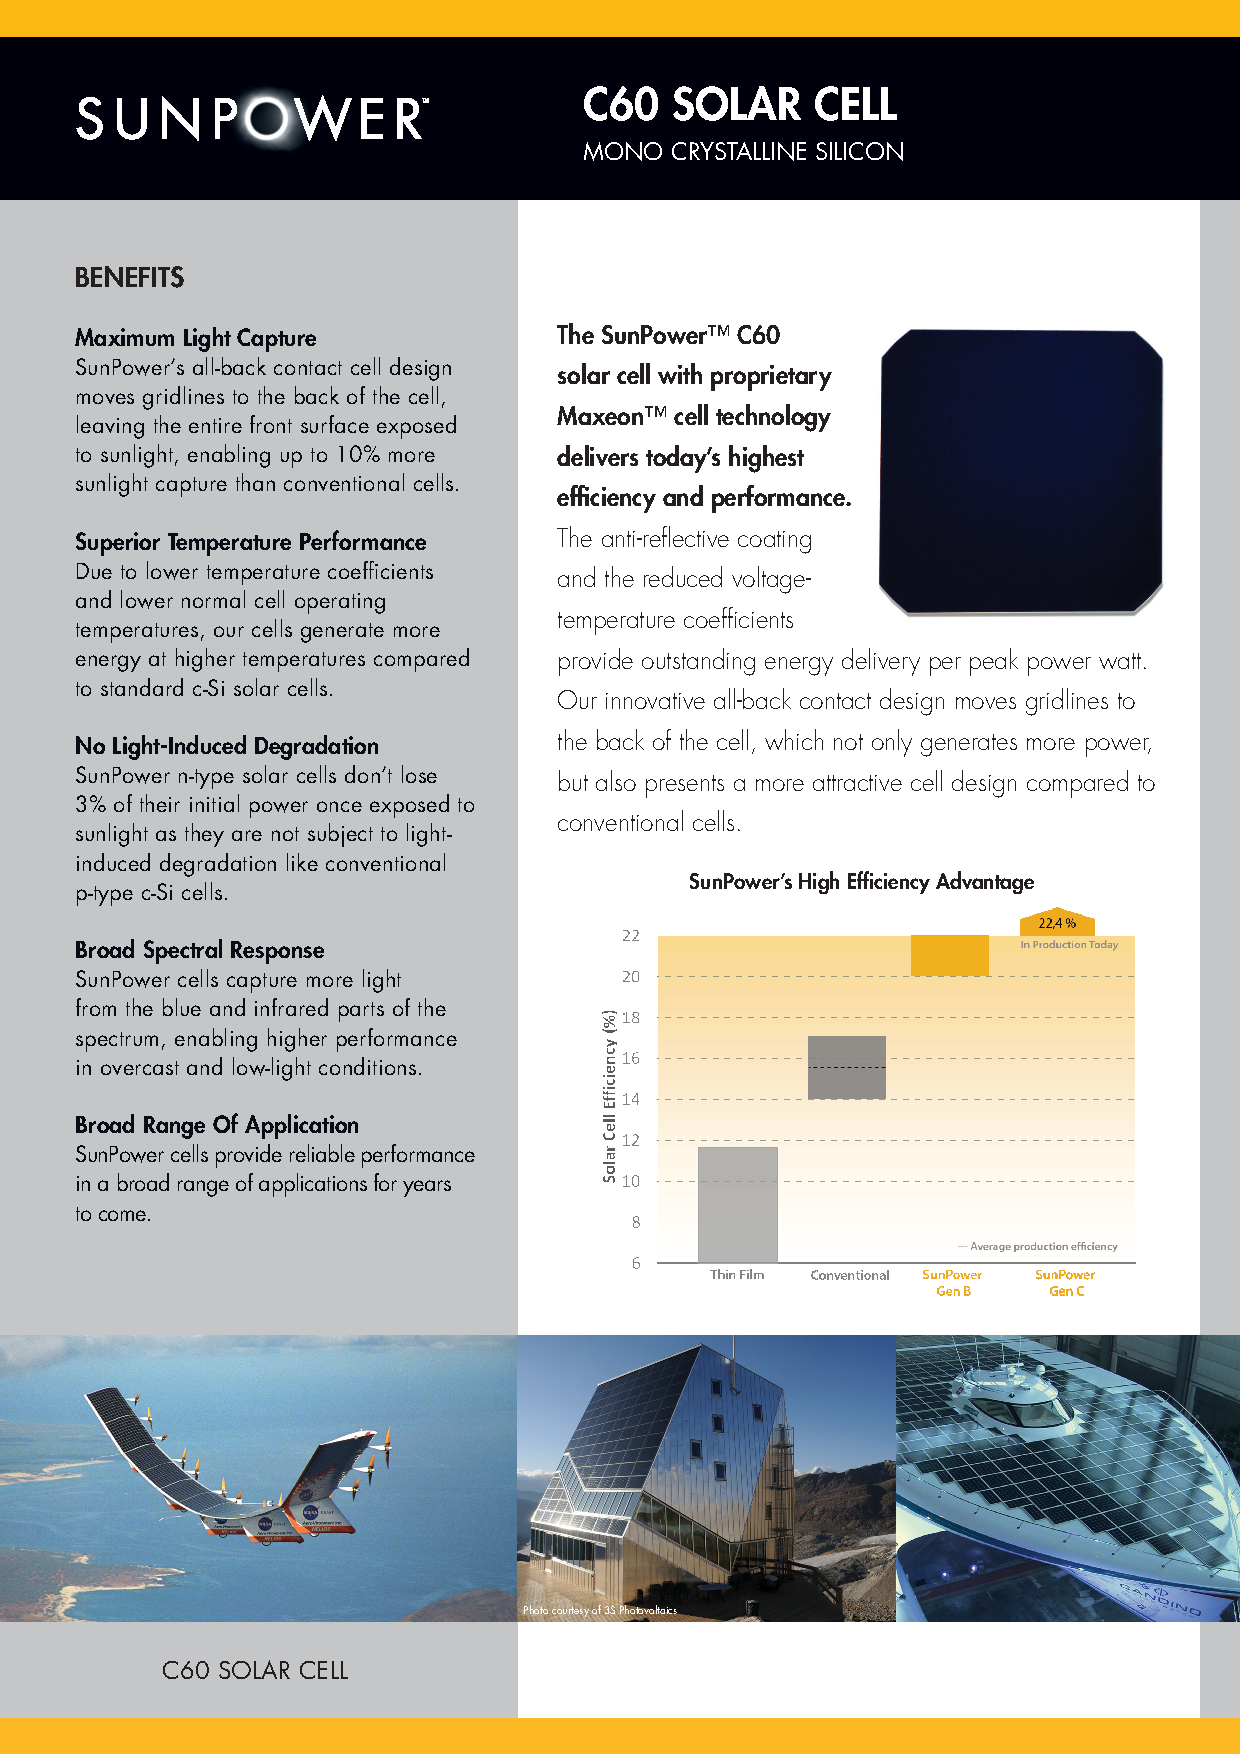
\includepdf[pages={1-2},nup=1x2,landscape=true]{Figures/SolarCell_Sunpower_C60.pdf}

 % file "Thesis_Appendix_B.tex"
%\cleardoublepage

% ----------------------------------------------------------------------
\end{document}
% ----------------------------------------------------------------------

